\documentclass[12pt,letterpaper, openany]{book}
\usepackage[utf8]{inputenc}
\usepackage{amsmath}
\usepackage{amsfonts}
\usepackage{titlesec}
\usepackage{amssymb}
\usepackage{makeidx}
\usepackage[usenames]{color}
\usepackage{graphicx}
\usepackage{caption}
\usepackage{Pgfgantt}
\usepackage{pdflscape}
\usepackage{hyperref}
\usepackage{tikz}
\usepackage{subcaption}
\usepackage[left=3.50cm, right=2.50cm, top=2.50cm, bottom=2.50cm]{geometry}
\author{Ricardo Fernández, Brami Prudencio, Juan Diego García}
\title{Desarrollo de un Sistema Interactivo con Body Tracking}
\begin{document}
	
\titleformat{\chapter}[display]{\normalfont\bfseries}{}{0pt}{\Huge}
\newpagestyle{mystyle}
{\sethead[\thepage][][\chaptertitle]{}{}{\thepage}}
\pagestyle{mystyle}
\begin{titlepage}
	\makeatletter
	\setlength{\@fptop}{0pt}
	\makeatother
\begin{figure}[t!]
	\centering
	
\includegraphics[width=8cm,height=5cm,]{./Images/Logo_Upb.png}
\end{figure}
\begin{center}
	\textbf{
		\large{UNIVERSIDAD PRIVADA BOLIVIANA\\
		FACULTAD DE INGENIERÍA Y ARQUITECTURA\\
		Ingeniería de Sistemas Computacionales\\[1cm]}
		\huge{PRÁCTICA INTERNA}\\[1cm]
		\Huge{Desarrollo de un Sistema Interactivo con Body Tracking}
	}\\[1cm]
\end{center} 
\textbf{Estudiantes: \\}
\textbf{
		Ricardo Fernández\\
		Juan Diego Garcia\\
		Brami Prudencio\\
	}
\begin{center}
		\textbf{
		Tutor:
		Ingeniero Marcelo Bernardo de la Rosa López\\[2cm]
	}
\end{center} 
	\begin{center}
		\textbf{Cochabamba, Diciembre 2020}
	\end{center}

\end{titlepage}
\@openrighttrue\makeatother
\tableofcontents
\makeatletter\@openrightfalse	
\listoffigures
\pagenumbering{arabic}\setcounter{page}{1}
\chapter{Resumen}


\chapter{Introducción}


\chapter{Objetivos}


\section{Objetivo General}

Desarrollo de un sistema interactivo con lectura de movimiento empleando una cámara y un computador personal para entrenamiento de posiciones, técnicas, baile, para uso personal en casa.

\section{Objetivos Específicos}

\begin{enumerate}
	\item Utilizar software existentes para el seguimiento corporal careciendo de una cámara de profundidad.
	\item Implementar una función para registrar mapas propios del usuario.
	\item Proveer una alternativa Open Source factible al mercado de sistemas interactivos con Body Tracking tales como Just Dance.
\end{enumerate}


\chapter{Estudio de Diagnóstico}


Esta propuesta nace del Sensei Inti Escobar, que dirige el Dojo Bushido Kai de Cochabamba, donde practico el arte marcial (Ricardo Fernández), es algo que me apasiona. Debido a la situación delicada del Corona Virus, los deportes han visto muchos problemas, entre ellos el Karate Deportivo necesita más opciones para evolucionar y adaptarse a estos cambios.
A partir de ahí, el Sensei Inti planteo la siguiente pregunta “¿Existe la posibilidad de que usando equipos tecnológicos podamos recrear un torneo de Kata de Karate?” y la respuesta sencilla es sí, pero es mucho más complicado que eso, después de investigar un poco, se plantea el uso de controles con sensor de movimiento, sin embargo, la disponibilidad y los precios dificulta su alcance. Debido a esto se plantea el uso de cámaras o Kinect.


1.- Debido a la situación delicada del Corona Virus, los deportes han visto muchos problemas, entre ellos el Karate Deportivo necesita más opciones para evolucionar y adaptarse a estos cambios.
2.- Esta propuesta nace del Sensei Inti Escobar, que dirige el Dojo Bushido Kai de Cochabamba, consiste en  Recreación de un torneo de karate no viable, por que
3.- Respuesta sencilla es sí, pero es mucho más complicado que eso, después de investigar un poco, se plantea el uso de controles con sensor de movimiento, sin embargo, la disponibilidad y los precios dificulta su alcance, ademas que pueden no soportar los movimientos bruscos.
4si .- Debido a esto se plantea el uso de cámaras o Kinect, sin embargo, kinect es un equipo caro que no tuvo grandes exitos, por lo que es normal que nadie vaya a usarlo, asi que se plantea el uso de camaras normales


Descripción estructurada detallada de la situación
problemática que origina la necesidad del proyecto
de grado.
10-20 paginas


\chapter{Marco Teórico}


El proyecto es un sistema interactivo que busca proporcionar al usuario independientemente de sus intereses, el cumplimiento de sus expectativas, siendo un desarrollo a conciencia, pero sin tomarlo demasiado en serio, busca también romper el estereotipo que imponen los proyectos de esta modalidad, que si bien, ofrecen un producto de relativa buena calidad y mantenimiento, son o bien productos comerciales como es el caso de Just Dance o productos privatizados como son los desarrollados para la medicina. 

En cambio, se tiene la expectativa de ofrecer al nivel de Open source del proyecto, que a la larga atraiga a más miembros, al igual que Linux o Apache y pueda expandir sus horizontes y calidad del producto, teniendo presente que Open Source no significa simplemente compartir el acceso al código fuente, como indica la \href{https://opensource.org/docs/definition.html}{Open Source Definition (OSD)}. 

El desarrollo del proyecto empleara los recursos disponibles y al alcance de cualquier desarrollador, por tanto, no tomara en cuenta el manejo de cámaras de profundidad, esta aclaración es necesaria, ya que la calidad del producto final puede ser muy variable al de proyectos similares y es una característica más por la que sobresaldría este proyecto, ya que reduciría el presupuesto necesario para el consumidor.\\

A continuación, se debe mencionar factores importantes sobre la implementación del proyecto, como las propiedades del Body Tracking, la verdadera forma que tiene esta herramienta que tiene para ofrecer al software, por que no sobra mencionar las distinciones entre una cámara normal y una de profundidad.


\section{Body Tracking/Motion Capture}

El seguimiento corporal del cuerpo, normalmente conocido como Body Tracking o Motion Capture hace referencia al seguimiento del cuerpo humano a través de una cámara, existen dos acercamientos a este estudio, el enfoque de ajuste del modelo y el enfoque de aprendizaje. El enfoque de ajuste del modelo involucra ajustar el modelo formulado según imágenes previas cargadas, estimando parámetros de puntos especificados de la imagen, sin embargo, es demasiado dependiente de extremos locales y la inicialización adecuada, lo cual lo vuelve inservible en ambientes nuevos. Este modelo comparte una similitud al método Monte Carlo basados en cadenas de Markov \cite{siddiqui2010human}.

En cambio, el enfoque de aprendizaje requiere de grandes cantidades de imagenes con notas y especificaciones del esqueleto en las imagenes, incrementando las dimensiones de espacio y memoria requerido. Un ejemplo de este tipo de reconocimiento es la herramienta PoseNet, derivado de TensorFlow, empleado para identificar objetos a partir de una base de datos propia que clasifique los elementos que se buscan identificar con silueta y nombre.

\begin{figure}[t!]
	\centering
	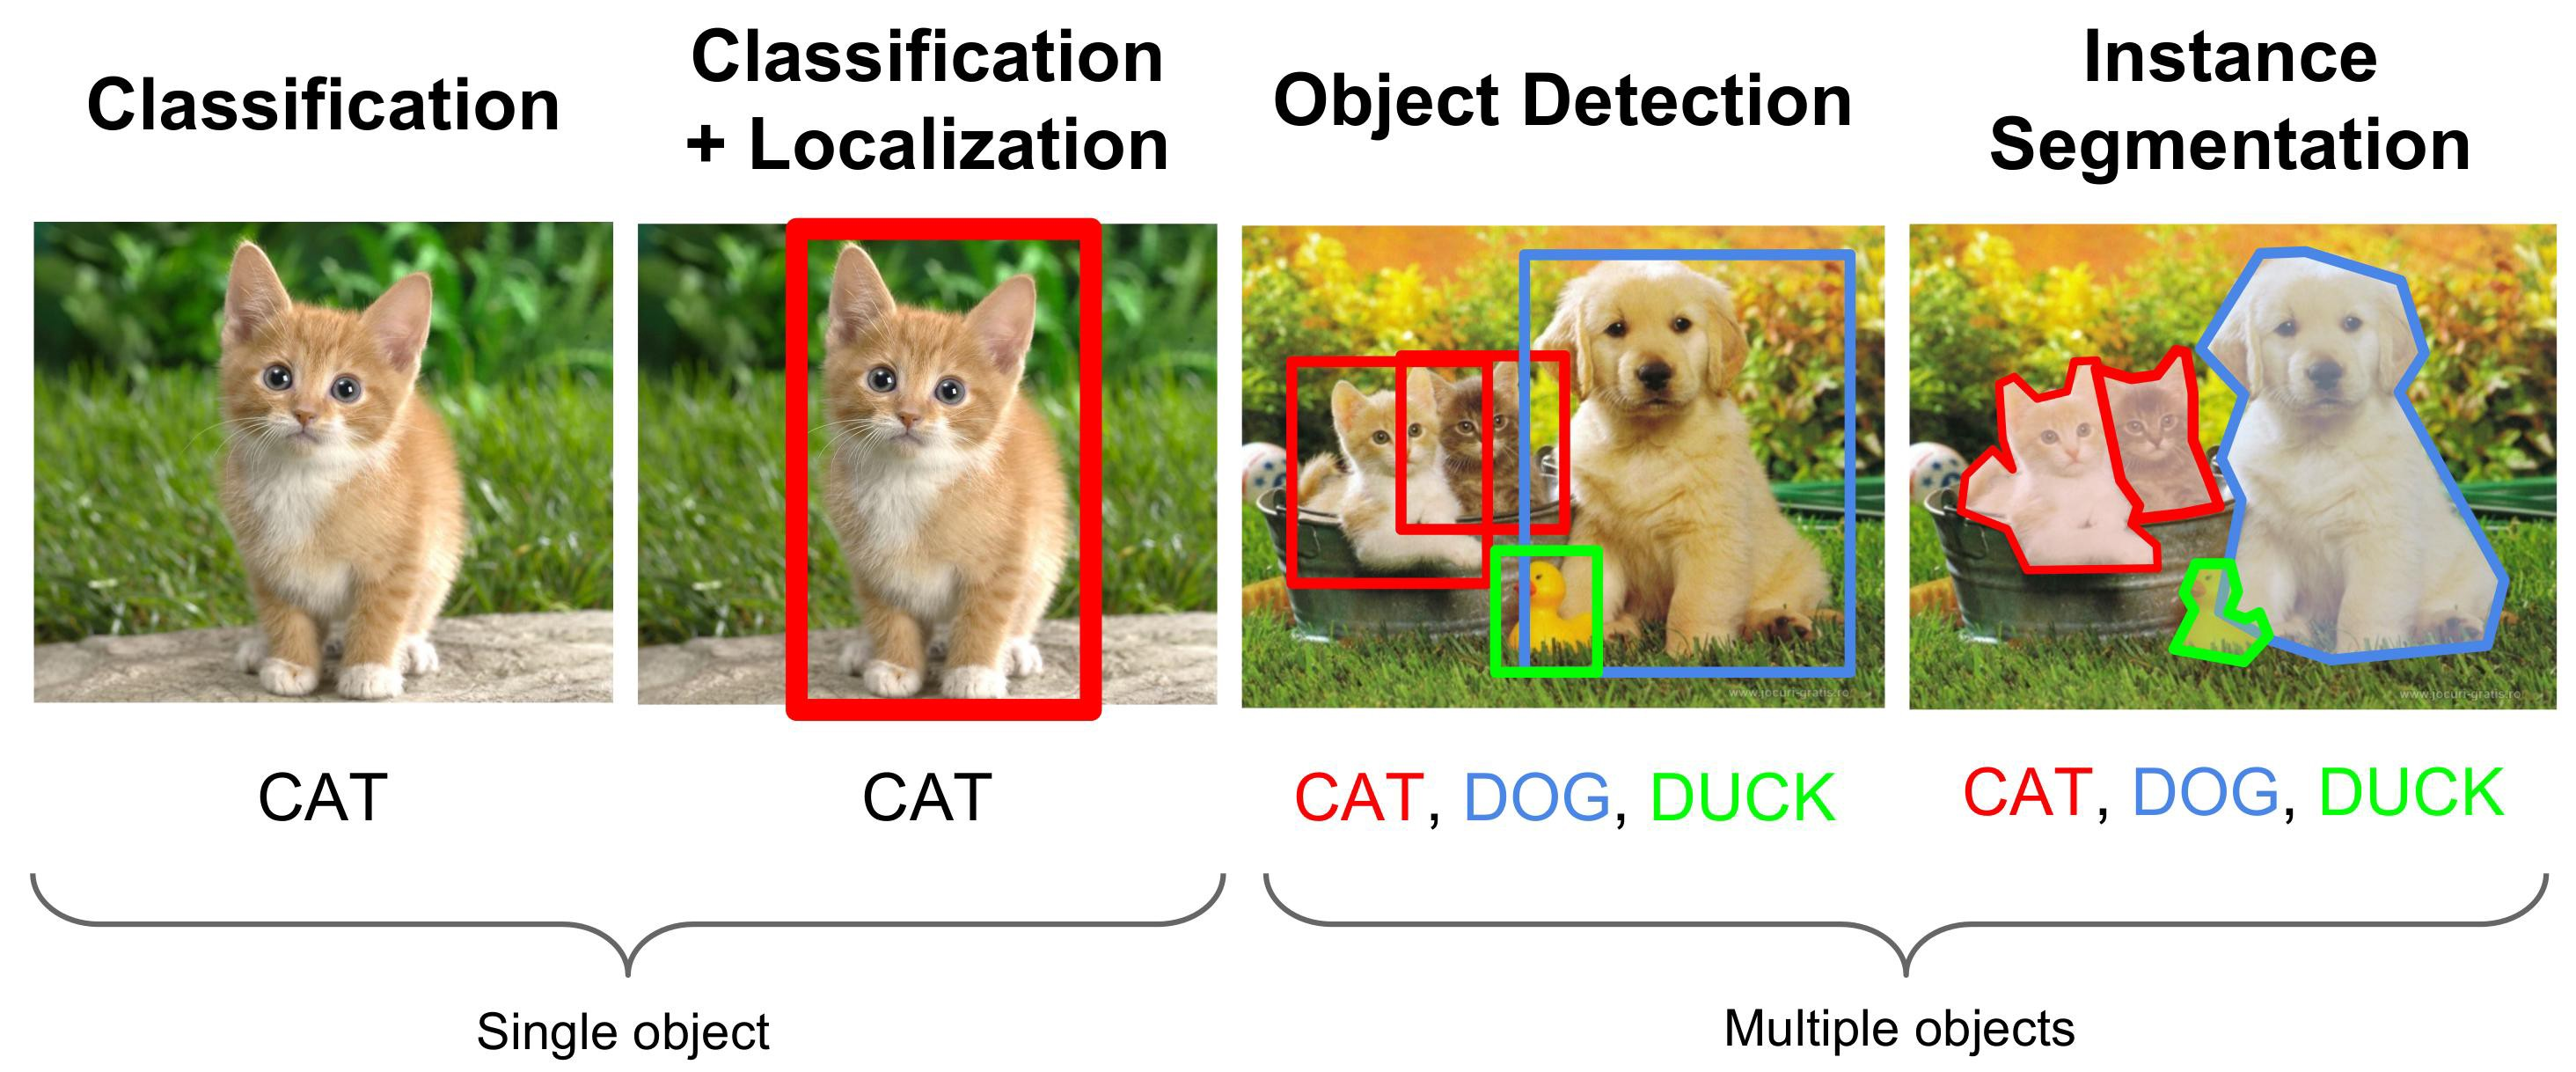
\includegraphics[width=13cm,height=5cm,]{./Images/ejemplotensorflow.jpg}
	\caption{Ejemplo de Clasificación de imagen de TensorFlow}
	\footnotesize Fuente: \cite{ejemplotensorflow}
	\label{tensorfl}
\end{figure}

Finalmente se empleo la iteración del punto más cercano \cite{grest2005nonlinear} el cual usa un enfoque de inicialización del esqueleto a través de fotogramas subsecuentes, clasificándolos con vértices y segmentos en un modelo 3D para este propósito.

La estimación de las poses humanas representan una problemática compleja de solucionar, el cual tuvo un largo trayecto hasta salir a la luz. La complejidad se centra en las múltiples limitantes, como las mascotas, los objetos del área, las personas de alrededor, la variación del escenario, los parámetros del cuerpo (el tamaño, longitud de las extremidades, torso y otras partes del cuerpo) y la iluminación.

Empleando las herramientas de seguimiento del Esqueleto, sensores de profundidad y sensores RGB, a medida que el tiempo corre, la necesidad de herramientas como los sensores va volviéndose obsoleta con el nacer de herramientas como PoseNet y OpenPose, que con el apoyo del Hardware mínimo necesario, son capaces de proporcionar la misma información con una calidad apenas inferior de seguimiento corporal.

\begin{figure}
	\centering
	\begin{subfigure}{.5\textwidth}
		\centering
		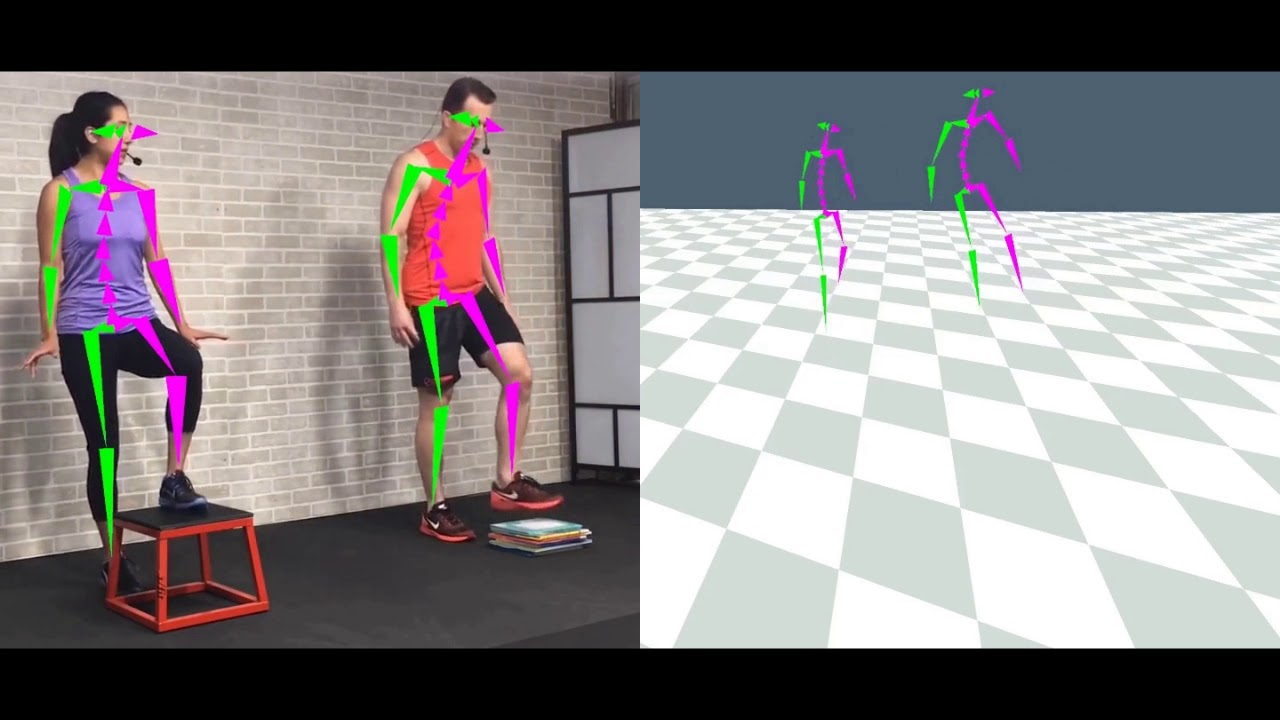
\includegraphics[width=8cm,height=7cm,]{./Images/examplebodytracking.jpg}
		\caption{Ejemplo 1}
		\label{bodyexa1}
	\end{subfigure}%
	\begin{subfigure}{0.5\textwidth}
		\centering
		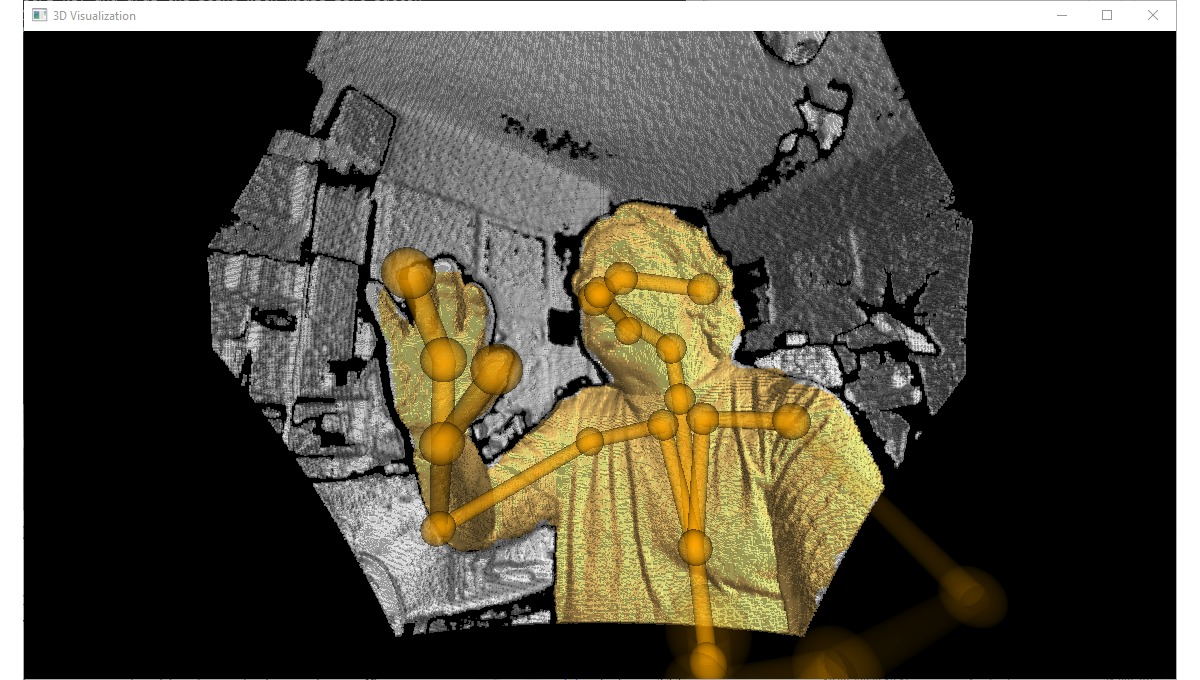
\includegraphics[width=8cm,height=7cm,]{./Images/examplekinect.jpg}
		\caption{Ejemplo 2}
		\label{bodyexa2}
	\end{subfigure}
	\caption{Ejemplos de Body Tracking}
	\footnotesize Fuente: \cite{examplebodytracking} \cite{examplekinect}
	\label{bodyexafigure}
\end{figure}

\subsubsection{Estimación de Poses}

La estimación de poses como su nombre indica, tiene la labor de estimar la pose de una persona a partir de modelos machine learning (ML) guardados en una base de datos, que proporcionan en ubicaciones especificas puntos clave que en su conjunto forman el esqueleto, además los datos sobre sus puntos se guardan como es explicado en el Análisis de Alternativas de PoseNet.

Se podría mencionar que su diferencia parte también de las palabras que lo conforman, Body Tracking/Capture Motion hace referencia a seguir el movimiento de una persona empleando Estimación de Pose, mientras que la Estimación de Poses hace referencia a marcar los puntos clave de una persona y construir un esqueleto de una persona \cite{oved2018real}.

\subsection{Skeletical Tracking}

Este fue una innovación brindada por el controlador Kinect al mercado comercial, Su demanda fue elevada en la época y hasta el día de hoy sigue siendo empleado, el reconocimiento de una persona desde cualquier angulo o distancia, tomando en cuenta su figura, tamaño, colo, cabello, ropa y el ambiente. Se emplea el escaneo de la imagen para reconocer puntos importantes del cuerpo que representan al cuerpo, tales como la cabeza, cuello, hombros, brazos, piernas y otros 10 a 20 puntos dependiendo la herramienta de reconocimiento que se emplee.


\begin{figure}[ht]
	\centering
	\begin{subfigure}{.5\textwidth}
		\centering
		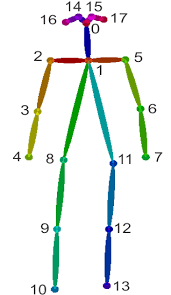
\includegraphics[width=4cm,height=6cm]{./Images/openposet1.png}
		\caption{Reconocimiento OpenPose Tipo COCO}
		\label{open1}
	\end{subfigure}%
	\begin{subfigure}{.5\textwidth}
		\centering
		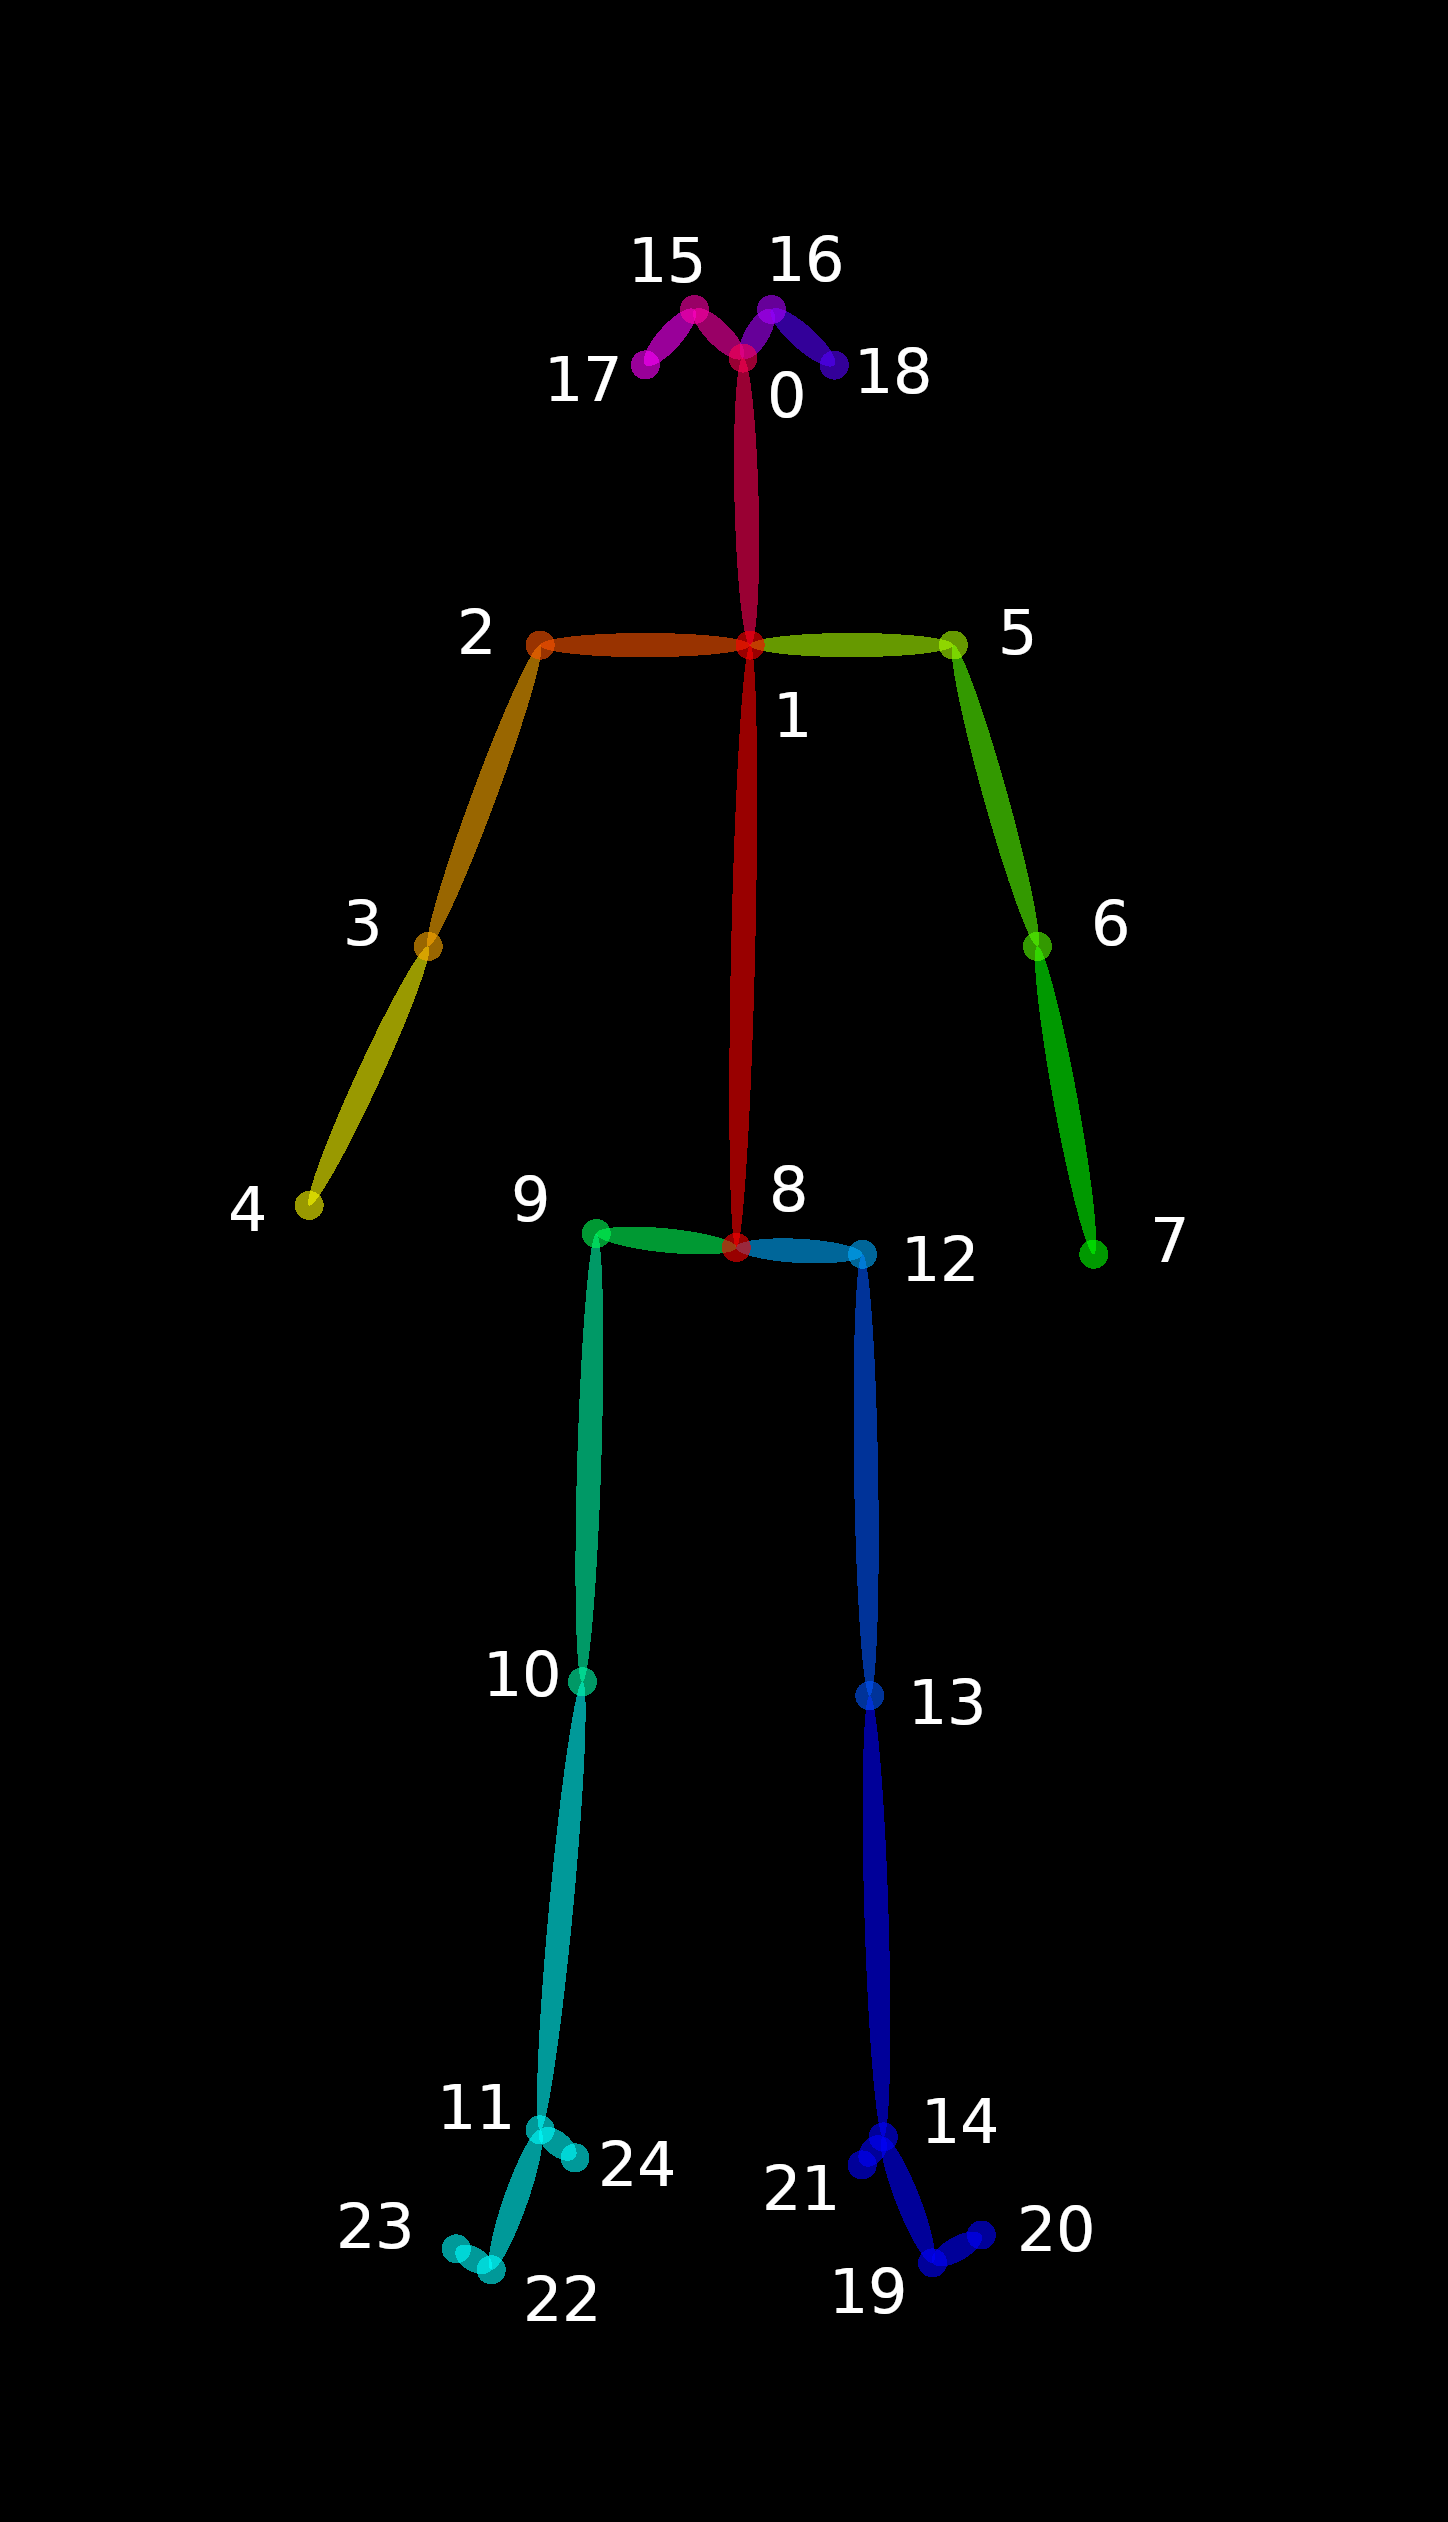
\includegraphics[width=4cm,height=6cm]{./Images/openposet2.png}
		\caption{Reconocimiento OpenPose Tipo BODY\_25}
		\label{open2}
	\end{subfigure}
	\caption{Diversos Tipos de Seguimiento al Esqueleto seleccionados por OpenPose para el desarrollo del proyecto}
	\label{exampleesqueletotrack}
	\footnotesize Fuente: OpenPose Models Image Output \cite{cao2017realtime} \cite{8765346}
\end{figure}

La herramienta seleccionada para el proyecto es OpenPose empleando este modelo de \href{https://github.com/CMU-Perceptual-Computing-Lab/openpose/blob/master/doc/output.md}{Formato de salida}, para los datos del seguimiento del esqueleto es emplear la flag write\_json para guardar la información dentro un JSON, el cual contiene un objeto de esqueleto de persona dentro, que contiene un vector pose\_keypoints\_2d con puntos 2D para localizar y detectar cada punto de unión x1,y1,c1,x2,y2,c2,.... Las coordenadas x y y en el rango de [0,1], [-1,1].

Además de la existencia de los vectores face\_keypoints\_2d, hand\_left\_keypoints\_2d y hand\_right\_keypoints\_2d, análogos a pose\_keypoints\_2d, los cuales debido a la masiva carga de memoria que requieren y la falta de ella (mínimo 4GB de Memoria dedicada estimada, contando solo con 2GB en el equipo proporcionado) serán ignorados, pero empleando pose\_keypoints\_2d.

Como dato, los vectores análogos body\_keypoints\_3d, face\_keypoints\_3d,
hand\_left\_keypoints\_2d y hand\_right\_keypoints\_2d (si --3d flag se habilitase), en vez de 
x1,y1,c1,x2,y2,c2,..., el formato sería x1,y1,z1,c1,x2,y2,z2,c2,..., donde c sería 1 o 0 dependiendo si la reconstrucción 3D es exitosa.

Se empleara el modelo BODY\_25 de Caffe, para mostrar el esqueleto, que consiste en mostrar 25 puntos del esqueleto, cada uno con su conexión en los siguientes puntos clave:

\begin{table}[t]
	\begin{center}
		\begin{tabular}{| c | c | c | c | }
			\hline Pos. & Punto Clave & Pos. & Punto Clave \\ \hline
			0 & Nariz&13 & Rodilla Izquierda \\ \hline
			1 & Cuello &14 & Tobillo Izquierdo \\ \hline
			2 & Hombro Derecho& 15 & Ojo Derecho \\ \hline
			3 & Codo Derecho & 16 & Ojo Izquierdo \\ \hline
			4 & Muñeca Derecha & 17 & Oreja Derecha \\ \hline
			5 & Hombro Izquierdo & 18 & Oreja \\ \hline
			6 & Codo Izquierdo & 19 & Dedo Gordo Izquierdo \\ \hline
			7 & Muñeca Izquierda & 20 & Dedo Meñique Izquierda \\ \hline
			8 & Cadera Central & 21 & Talón Izquierdo \\ \hline
			9 & Cadera Derecha & 22 & Dedo Gordo Derecho \\ \hline
			10 & Rodilla Derecha & 23 & Dedo Meñique Derecho\\ \hline
			11 & Tobillo Derecho & 24 & Talón Derecho \\ \hline
			12 & Cadera Izquierda & 25 & Escenario \\ \hline
		\end{tabular}
		\caption{OpenPose Output JSON Content, Which are Given X, Y and C values}
		\footnotesize Fuente:\cite{8765346}
	\end{center}
\end{table}


En cuanto al resultado, este se puede guardar en formatos estándar (JSON, XML, PNG, JPG,...), existen suficientes herramientas de uso libre para leerlos, por tanto cargar los datos y cargar las imágenes, no debería representar un desafió.

\section{Base Teórica}

\subsection{Cámara y Desambiguación}

Una cámara se define como un dispositivo que permite el registro y reproducción de imágenes. A través del tiempo, se desarrollaron muchos tipos de cámara, por tanto es necesario determinar el tipo de cámara del cual se dispone para la elaboración del proyecto, siendo el selecto la cámara Web. Sin embargo, en la mayoría de proyectos relacionados al Body Tracking, se menciona el termino Depth of Field (DOF), mención a una cámara de profundidad de campo.

La cámara web es un modelo pequeño de una cámara digital conectada a una computadora. Tiene la capacidad de capturar imágenes y transmitirlas a través de Internet. Un punto importante es que pueden ser empleadas para el desarrollo de aplicaciones y programas de cierta índole. 


\subsubsection{Depth of Field (DOF)}

La profundidad de campo es el producto del deseo de producir una imagen más clara del objeto o escenario deseado. Normalmente, una cámara debe enfocar su lente para tener mayor precisión, por tanto, se adjuntaron formas para ajustar el lente. Actualmente, se desarrollaron sistemas automáticos para el ajuste del lente, los cuales incluyen la medición de la distancia al objetivo, empleando esta para ajustar el lente y obtener mayor claridad \cite{madsen2000depth}. 

\subsubsection{Sensores RGB-D} 

Es el termino dado al conjunto de sensores RGB y Depth (de profundidad).Los sensores de RGB y profundidad son una adición a los dispositivos como Kinect, PlayStation Camera y otros. 
\\El sensor de profundidad cumple la función de proyectar luz infrarroja y un sensor infrarrojo. 

Divide su funcionalidad en dos pasos, la proyección de rayos de luz infrarroja, los cuales rebotan en el ambiente en el que se encuentra y posteriormente son detectados por el sensor de infrarrojo. Esta información es decodificada y enviada al usuario para poder emplearla como se lo estime.
\\
RBG es un modelo de colores basado en la obtención de un color empleando una mezcla entre otros colores, todas ellas con los colores primarios, que son el rojo, verde y azul. 
El sensor RBG analiza el escenario que tiene en frente, determinando la cantidad de luz que requiere la producción de una imagen de calidad, optimiza y ajusta la velocidad de obturación, apertura y sensibilidad de captura de luz. 
Se encarga de analizar cada pixel del Frame y crear una imagen meticulosa.
\\
En el desarrollo del proyecto, no se empleara un sensor de profundidad, ya que una cámara Web no lo tiene equipado.

La funcionalidad del sensor RGB-D es combinar la información colectada por el sensor infrarrojo y el sensor RGB, proporcionan datos de color y profundidad a cada pixel en cada Frame que analiza. Dentro de la memoria del Kinect, existen patrones de referencia, que poseen colores y profundidades ya conocidas, que facilitan la estimación del escenario que lo necesite\cite{litomisky2012consumer}.  
\begin{figure}[t!]
	\centering
	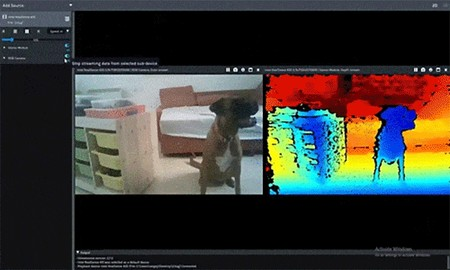
\includegraphics[width=10cm,height=6cm,]{./Images/RGBandDepth.jpg}
	\caption{Ejemplo de Visión de una Cámara con sensores RGB-D}
	\footnotesize Fuente: \cite{RGBandDepth}
	\label{RGBandDepth}
\end{figure}


\subsection{Inteligencia Artificial (IA)}

Una faceta importante del proyecto, es la estimación de poses, elemento producto de la Inteligencia Artificial y Machine Learning, si bien, es explicado en la sección de PoseNet.
\\
La inteligencia artificial (IA) es una rama de la ciencia de computación, que se define como "Un programa que en un mundo arbitrario, no se las arregle peor que un humano"\cite{dobrev2012definition}. 
Esta definición se somete a muchos factores, para empezar requiere de asumir tres factores importantes.
El primer factor es que cualquier dispositivo de calculo puede ser modelado por un programa. El segundo factor es que el IA es un dispositivo que permite ingresar información de afuera y dar una respuesta de acuerdo a ello. El tercer factor es asumir que la IA, al estar en contacto con el mundo este recibe información que da una respuesta interactiva con el mundo. Se asume que el mundo en que se encuentre será influenciado por la IA\cite{dobrev2012definition}. El mundo se considera como el ambiente con el que la IA tiene interacción, aquel que proporciona los valores que la IA procesará y aquel que reaccionará a las acciones y/o valores de salida de la IA, en un proceso de emisión y recepción continuo.

\subsubsection{Machine Learning (ML)}

El aprendizaje de la máquina o Machine Learning es ua rama de la ciencia de computación dirigida en algoritmos Computacionales diseñada para emular la inteligencia humana, a través del aprendizaje del mundo que lo rodea.

Los modelos ML ganan popularidad debido a su capacidad de proporcionar resultados y conocimientos de un tipo especifico en escenarios similares a los que ha entrenado, pero nunca antes visto. Los modelos ML provee información relevante sobre los datos relacionados a lo que se requiere, traduciendo los datos de entrada, en datos que se desean obtener. Por ejemplo, un médico, para diagnosticar a un paciente con un síntoma tan común como fiebre, requerirá de un extenso conocimiento en enfermedades que tienen este síntoma y basándose en todo su conocimiento teórico, indagara en información que pueda relacionar con la fiebre, especificando otros problemas o falta de ellas que tenga y llegará a una conclusión sobre que enfermedad padece \cite{murdoch2019interpretable}.

Una versión simplificada es decir que Machine Learning emplea algoritmos para clasificar y filtrar la información recibida, aprender de ella, guardarla y tomar una decisión basándose en lo aprendido. 

\subsubsection{Deep Learning (DL)}

El aprendizaje profundo o Deep Learning es una subrama de Machine Learning que se basa en el uso de Neural Network, empleando numerosas capas y nodos para el aprendizaje, que en conjunto a toda la base de datos previa da lugar las decisiones en las que se basa.

El Deep Learning utiliza múltiples capas de decisión, siendo el dato de ingreso interpretado por el logaritmo en diferentes niveles, cada uno repercute en el anterior y produce un aprendizaje basado en intento y error para aprender, corrigiendo los datos de salida de cada capa para llegar a una respuesta cada vez más aproximada a la deseada.
Una diferencia importante entre Machine Learning y Deep Learning, es que, Machine Learning en general mejora con el tiempo, pero requiere de corrección de vez en cuando, si se desvía de los resultados que se buscan.En cambio, Deep Learning determina si su propia predicción es correcta haciendo uso de su red neuronal, no requiere de intervención.
\\
En el desarrollo del proyecto se hace mención al modelo CAFFE y COCO, los cuales son parte fundamental en el proyecto, ya que estas son los modelos de Deep Learning empleados para el Body Tracking.

\subsubsection{Modelo DL CAFFE}

El modelo CAFFE es un Framework opensource trabajado con las librerias C++ y CUDA para Deep Learning, tiene interfaces en Command Line, Python y MathLab, incluye soporte en problemas con el modelo, tiene referencias, demos y herramientas para poder usarlo, además de la caracteristica de usarse con CPU y GPU\cite{jia2014caffe}.

Además de poseer una comunidad abierta a ampliar el desarrollo y trabajar con la herramienta, ventaja caracteristica del codigo open source. 
El modelo CAFFE ofrece el poder definir modelos, optimizar opciones para el desarrollo y pre-entrenar para poder realizar el aprendizaje.

En la sección del proyecto, CAFFE realizo sus estudios para poder guardar Dataset de miles de cuerpos humanos, otorgándole puntos clave para formar el esqueleto. 
La herramienta OpenPose selecta hace uso de la CMU Panoptic Dataset, que junto a  sus miles de miles de esqueletos 3D permite estimar la pose humana, produciendo el Modelo BODY\_25 visto previamente en la figura \ref{open1}.

\subsubsection{Modelo DL COCO}

EL modelo COCO es un Dataset reciente del año 2014, desarrollado para el reconocimiento de objetos en el contexto requerido, a través de la obtención de imágenes complejas que contengan la información requerida en su estado natural.
En su mayoría, posee objetos reconocibles por niños pequeños, tiene 2.5 millones de etiquetas en mas de 300000 imágenes.

En el contexto, el modelo COCO posee miles de imágenes relacionadas a la identificación del cuerpo humano y la construcción de su esqueleto, marcando con etiquetas sus puntos claves del cuerpo y la confiabilidad de esos datos\cite{lin2014microsoft}.

\subsubsection{Neural Network}

Neural Network inicialmente es inspirado por la compleja red de neuronas del cuerpo humano, el cual transmite información, ordenes a través de impulsos eléctricos, donde miles de millones de conexiones existen, con ese fin\cite{wang2003artificial}. 
\\

Formalmente, el modelo de Neural Network consiste en un set de unidades Computacionales y un set de conexiones de una vía unidas. A través del ingreso de datos, las unidades Computacionales lo examinan y computan, generando una activación como dato de salida. La activación atraviesa la conexión que tiene la unidad Computacional con otra unidad y procede a examinarlo y computarlo para generar otra activación. 
Este proceso se repite, con el fin de aumentar el llamado peso que determina la influencia que se obtiene al examinar y computar el valor recibido, dependiendo el objetivo, mientras mayor o menor termine siendo el peso en las conexiones a medida que se computan las activaciones en las unidades Computacionales, mayor efecto tendrá en el dato de salida. 
Un ejemplo de ello se observa en la figura \ref{neuralnetwork} \cite{gallant1993neural}, donde los círculos representan unidades Computacionales, las flechas las conexiones, los valores los pesos, ingreso de datos es el 1 y el dato de salida es 0. El 0.73, 0.79 y 0.69 es el resultado de una Activación después del primer computo.
\\
Esta herramienta es empleada por OpenPose y PoseNet para el entrenamiento de las herramientas de estimación de pose, que lo utilizan para que con los Dataset de miles de imágenes que sirven como imágenes de ingreso y sus etiquetas, puedan ser analizadas por extensas capas de unidades Computacionales que evaluaran cada imagen y proporcionaran pesos, que a mayor peso, mayor precisión en la estimación de pose tendrá.
\begin{figure}[t!]
	\centering
	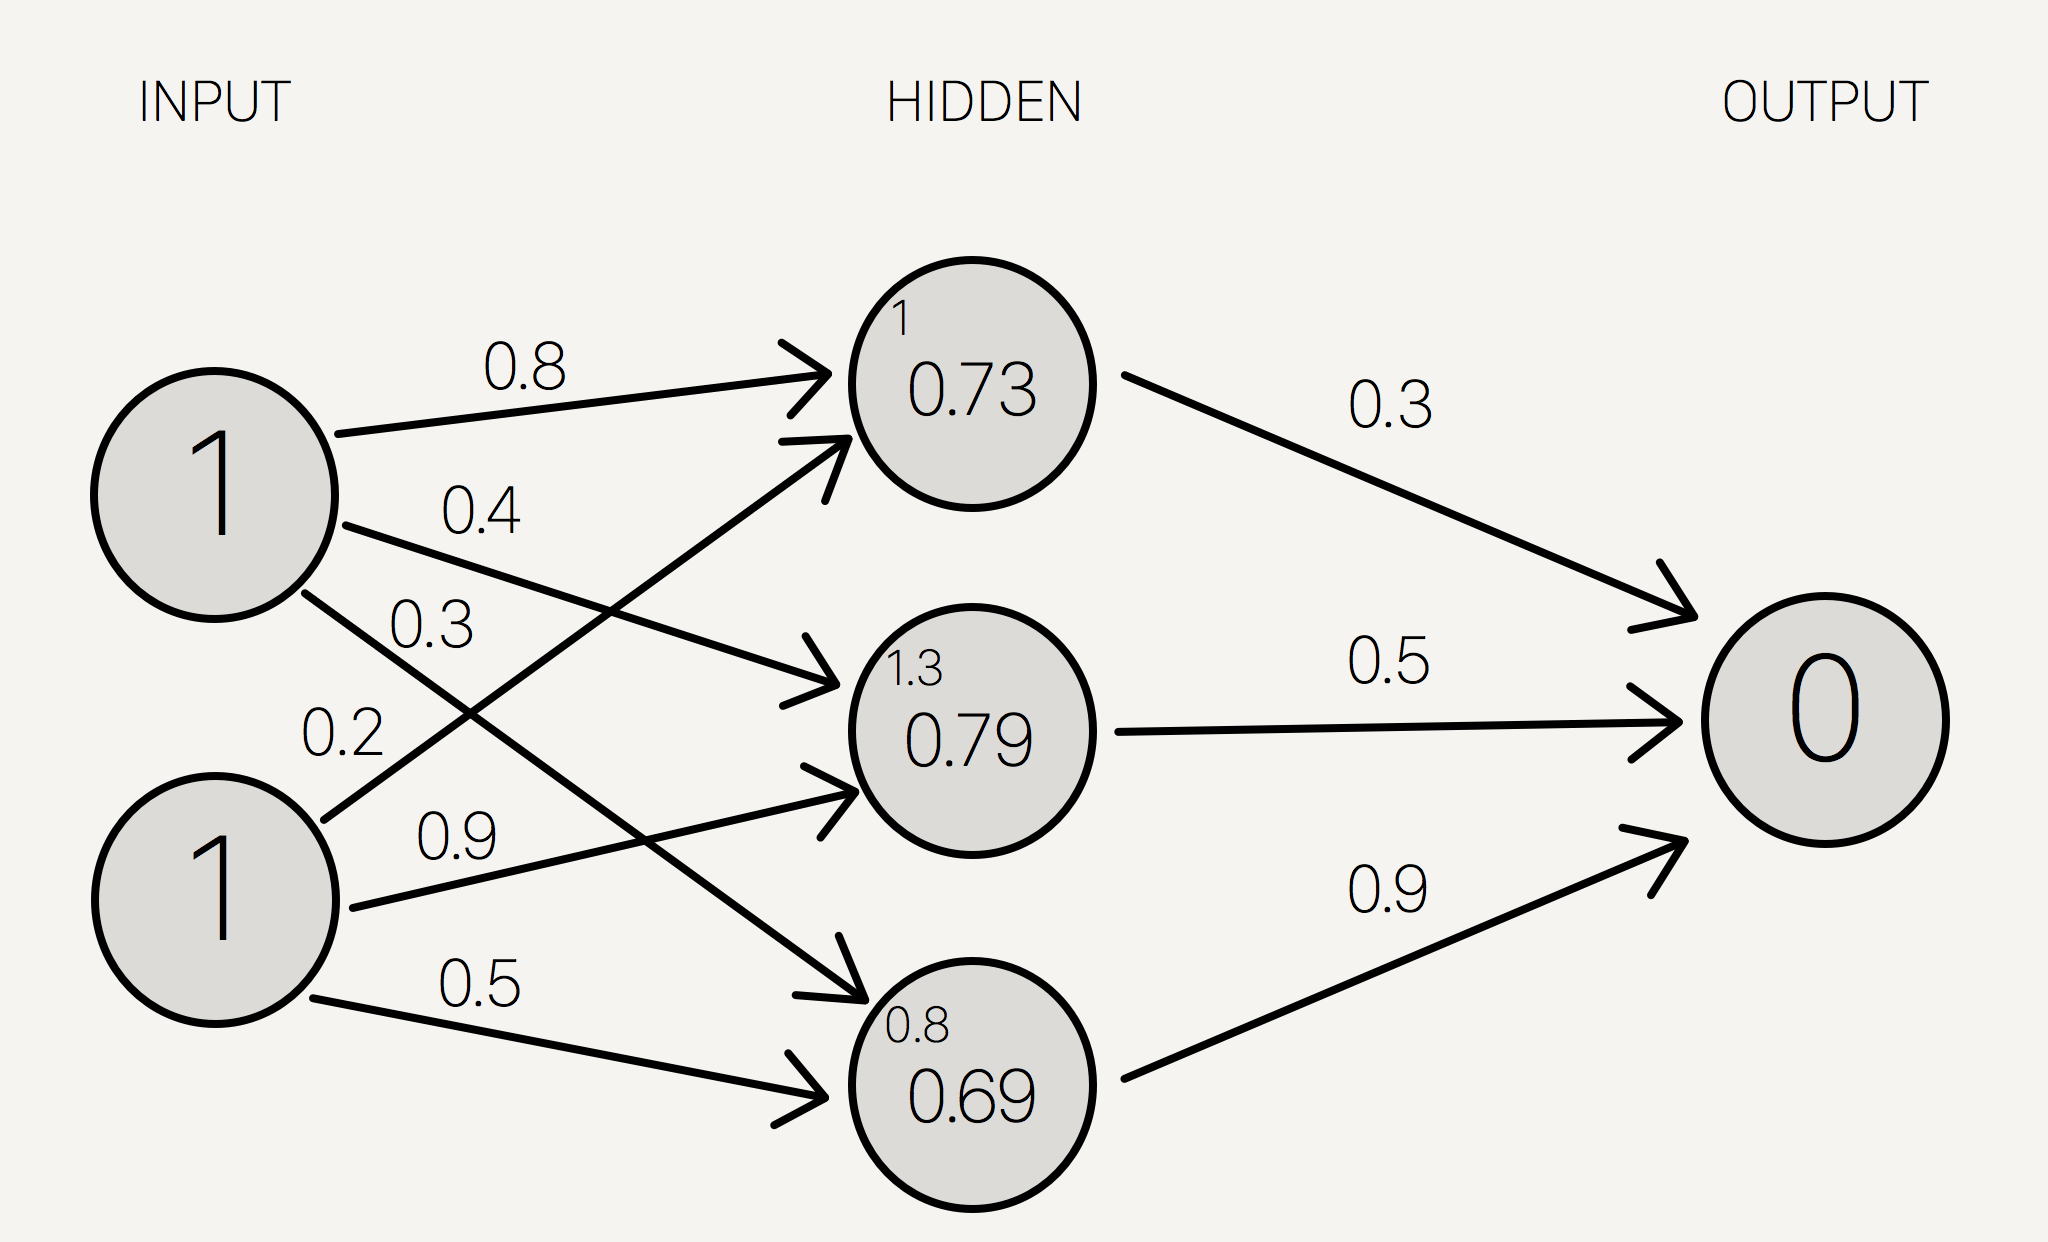
\includegraphics[width=11cm,height=5cm,]{./Images/neuralnetwork.png}
	\caption{Ejemplo de Neural Network}
	\footnotesize Fuente:\cite{8765346}
	\label{neuralnetwork}
\end{figure}
\chapter{Estudio de alternativas}

\section{Análisis de Alternativas actualmente disponibles en el mercado}

En la actualidad, en la extensión de la investigación, existen productos comerciales y proyectos privados que se asemejan a las características ofrecidas por el proyecto, son en su mayoría de índole privatizada especialmente en el campo de la medicina, donde solo se hace mención a sus resultados, sin embargo, ninguna resalta por su accesibilidad gratuita, distinguiendo el proyecto del factor común. Siendo las aplicaciones y programas desarrollados con un enfoque principal en entretenimiento, como es el caso de videojuegos y medicina, en analizadores médicos y programas de rehabilitación.\\

\subsubsection{Analizadores Médicos}

En la rama de la medicina, la información es más privatizada o proporciona un menor alcance al publico, solo reporta resultados y posibles cambios y amplitudes afirmando la falta de pruebas para dar mayor información, por lo que profundizar en ello no otorgara profundidad al proyecto, no obstante, se ha encontrado que se utiliza la tecnología planeada para controlar la pose del usuario, ya sea en pruebas médicas para hallar anormalidades físicas en la posición del cuerpo al realizar diversas actividades y en entrenamiento físico para mantener una posición estable y evitar dañarse a uno mismo.

\subsection{Entretenimiento}

Cuando se referencia a un sistema de estimación de pose del cuerpo, se nombran varios títulos de videojuegos de baile, siendo las primeras y más importantes sagas, las desarrolladas por Ubisoft como Just Dance o Dance Experience, enfocadas en realizar coreografías pre-diseñadas para canciones populares en la época del lanzamiento de sus entregas; a pesar de que en Just Dance han existido niveles con temática de artes marciales, estas no contaban con la intención de ser un entrenamiento educativo, sino un baile con el propósito de entretener utilizando movimientos basados del arte marcial.  \\
\\
Además de las mencionadas, existe otro género en los videojuegos enfocado al entrenamiento físico, como Shape Up de Ubisoft y Wii Fit de Nintendo, estas enfocadas más a un entrenamiento físico casual como es el caso de Shape Up, donde se incentiva al jugador a realizar ejercicios anaeróbicos de alta intensidad como son flexiones, abdominales o sentadillas y Wii Fit enfocado a rutinas de Yoga, equilibrio y aeróbicos; demostrando las diferentes aplicaciones y posibilidades de desarrollo y resultados. \\

\subsubsection{Just Dance}

Just dance es una serie de sistemas interactivos con Body Tracking, es un producto pionero en el tema desarrollado por Ubisoft París que debuto en octubre del 2010. La serie de Just Dance cuenta con un total de 30 títulos con un amplio rango de categorías de edades para llegar a la audiencia, es ya una serie que libera un nuevo titulo al menos una vez al año, demostrando ser un éxito comercial. Gran parte de la inspiración del proyecto actual es este sistema interactivo, que emplea al máximo el controlador Kinect y el Body Tracking con comandos de voz para ofrecer un uso casual y entretenido, sin embargo, la carencia del equipo y la frustración de no ser capaces de aprovecharlo, se desvían en cambio a la posibilidad de crear una alternativa, el cual se espera que con el equipamiento provisto para el proyecto, carente de una cámara de profundidad (elemento sobresaliente en el controlador Kinect), permita el desarrollo adecuado de las características de Body Tracking.


\section{Análisis de Alternativas En Herramientas Disponibles Para el Desarrollo}

\subsection{Trajes con sensores de movimiento}

La industria actual de cine, sistemas interactivos, deportes e incluso la medicina cuentan con una inversión que llega a niveles millonarios en recrear animaciones del cuerpo humano, empleando las herramientas externas que faciliten la lectura de movimiento, su uso es bastante extendido y llega a crear obras de gran calidad, sin embargo, en su mayoría esta tecnología no esta disponible para el publico en general debido a su elevado costo, y ya que no es un campo prioritario de investigación en la Universidad Privada Boliviana, por tanto, esta alternativa queda descartada.
\\
Los trajes cuentan con 19 sensores distribuidos alrededor del cuerpo y recogen movimientos de un actor para transmitirlos en tiempo real. Una de sus ventajas es la reducción de costos en las producciones para motion capture, además de no requerir un set de estudio demasiado restrictivo para su implementación. Existen además, varios modelos del traje proporcionados por empresas como Xsens, Holosuit, Teslasuit y otros.

\begin{figure}[t!]
	\centering
	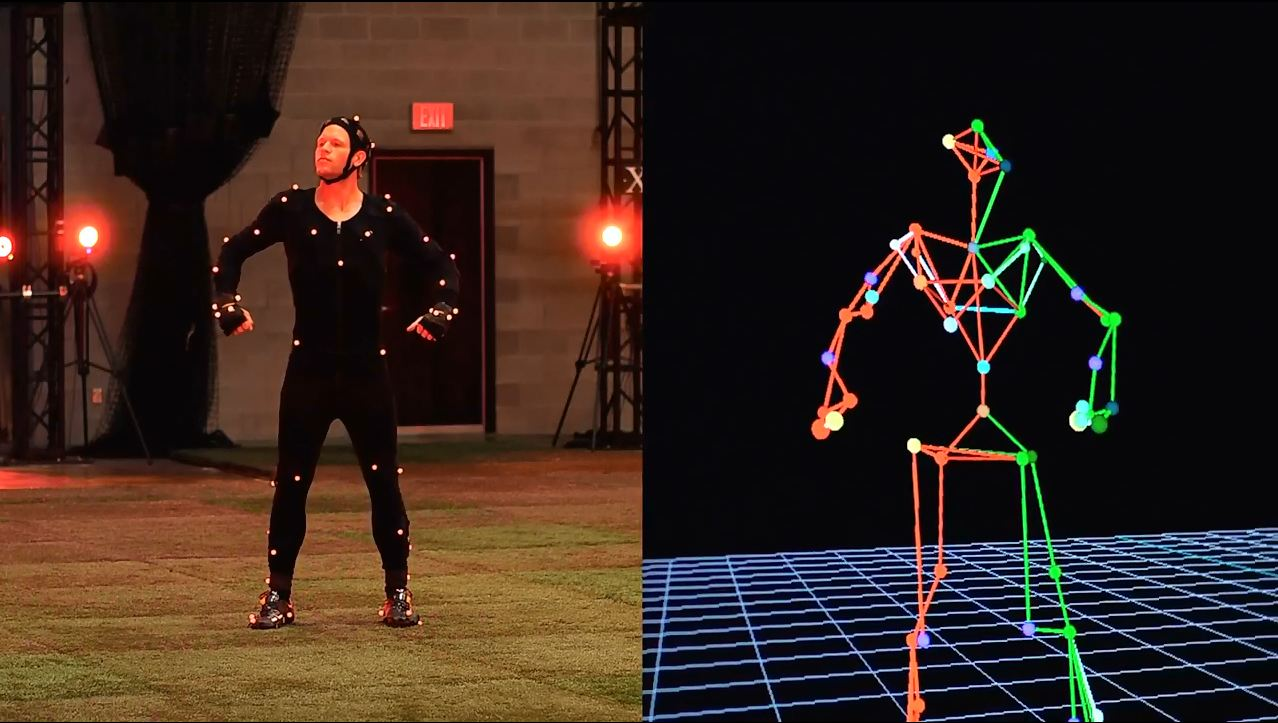
\includegraphics[width=9cm,height=4cm,]{./Images/trajesensor.jpg}
	\caption{Traje con Sensores de Movimiento}
	\footnotesize Fuente: \cite{trajesensor}
	\label{trajesensores}
\end{figure}

\subsubsection{Creación de Software propio para Body Tracking}

Uno de los objetivos implícitos del desarrollo de este proyecto es el siguiente "El objetivo no es volver a crear la rueda, sino, crear algo nuevo utilizando esa rueda", palabras del supervisor del proyecto, por tanto, a pesar de ser un posible acercamiento a la solución, queda completamente descartada.

\subsection{TensorFlow}

\href{https://www.tensorflow.org/lite/models/pose\_estimation/overview}{Tensorflow} 
es una herramienta open source para Machine Learning provista de soporte por Microsoft, la comunidad la ha empleado extensamente en proyectos y estudios de múltiples campos de la inteligencia artificial,  de Body Tracking con el uso de PoseNet, derivado de TensorFlow, cuenta con soporte y una documentación clara, siendo además sus requisitos recomendados para su uso relativamente bajos. 
\\
TensorFlow se basa en redes neuronales para Deep Learning, es una herramienta interfaz que implementa algoritmos para Machine Learning, puede ser ejecutada con una variedad de sistemas, desde celulares hasta Tablets, e incluso sistemas a gran escala. Tiene un amplio rango de algoritmos de entrenamiento, incluyendo entrenamiento e modelos de inferencia para Neural Network Models e investiga ramas de múltiples ramas, incluyendo recolección de información, proceso de entendimiento de un lenguaje natural, geografía, descubrimiento de drogas, ciencias Computacionales y otros.  \cite{abadi2016tensorflow}

\subsection{PoseNet}

PoseNet es una herramienta desarrollado por Google Creative Lab basada en TensorFlow que permiten demostrar una estimación a tiempo real de estimación de poses (Body Tracking) en tiempo real. Esta herramienta puede ser empleada tanto para una persona a la vez como para varias personas a la vez dependiendo del algoritmo que se emplee, la diferencia es en la velocidad y simpleza en su función \cite{kendall2015posenet}.
\\
Debido a que el proyecto será para un uso singular, se mencionara su posibilidad a través del algoritmo (del cual se desconoce su funcionamiento interno, ya que no es explícitamente necesario para el proyecto, es parte de una herramienta que se empleará) de Body Tracking para una persona.

Emplea una imagen RGB que alimenta a la red neuronal y emplean un decodificador de poses, designando valores de confianza, posiciona puntos clave y valores de confianza para los puntos clave para el aprendizaje de la red neuronal en la lectura de imágenes con las cuales aprendió a estimar las posiciones en tiempo real\cite{oved2018real}.
\\
En cuanto los términos previos, son propios de la estimación de pose, por tanto se los debe explicar y mostrar visualmente para su entendimiento, los cuales se denotan en la figura \ref{exampleposenet}:

\begin{itemize}
	\item Pose: Retorna un objeto que contiene una lista de puntos clave y valores de confidencia para cada persona detectada.
	\item Valor de confianza de pose: Determina la confianza que tiene la estimación de la pose,en un rango de 0 a 1 y puede ser usado en caso que las partes del cuerpo bloqueadas por el cuerpo mismo o elementos externos represente un obstáculo para su lectura exacta.
	\item Punto Clave: Son literalmente un grupo de puntos, es la parte que se estima del cuerpo humano para formar el esqueleto, como se observa claramente en la figura \ref{open2}. En la base de datos de modelo COCO, existen 17 puntos de lectura.
	\item Valor de Confianza de un punto clave: Determina en un rango de 0 al 1 la confianza que se tiene de la precisión del punto determinado, bajo el mismo concepto de la pose, en caso que existan obstáculos.
	\item La posición del punto clave: Las coordenadas (x,y) de la imagen en las que se encuentran los puntos claves.
\end{itemize}

\begin{figure}[ht]
	\centering
	\begin{subfigure}{.5\textwidth}
		\centering
		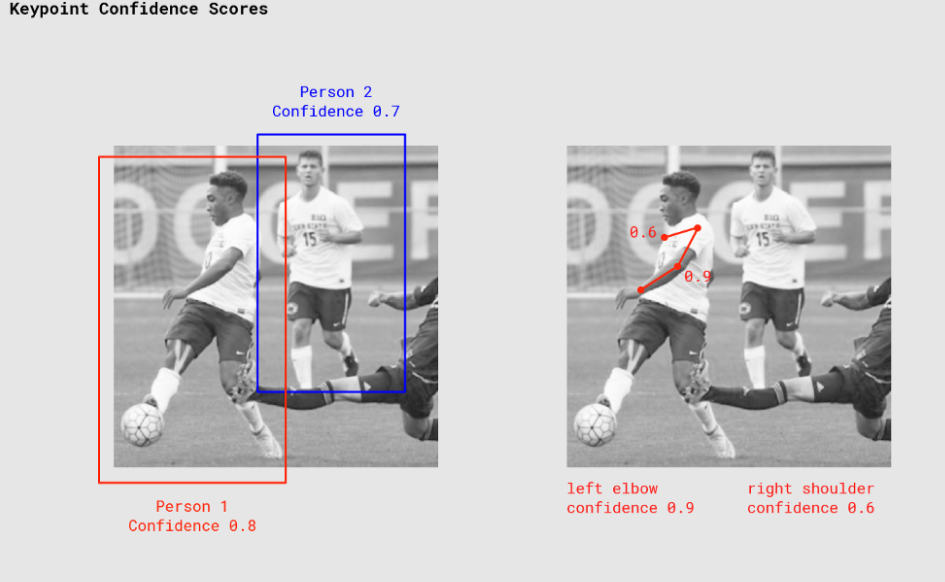
\includegraphics[width=7cm,height=5cm,]{./Images/posenetcocoexample.png}
		\caption{Ejemplo a}
		\label{posenet1}
	\end{subfigure}%
	\begin{subfigure}{.5\textwidth}
		\centering
		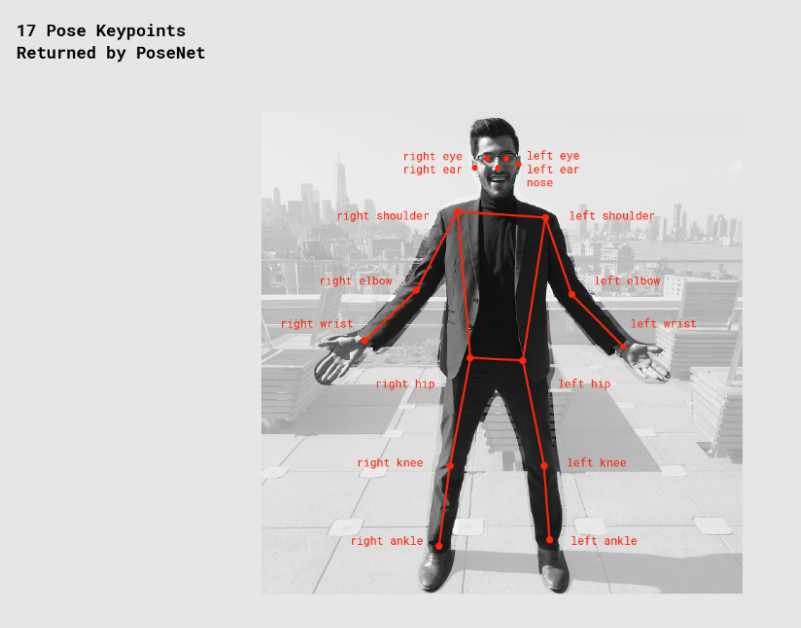
\includegraphics[width=7cm,height=5cm]{./Images/posenetexample2.png}
		\caption{Ejemplo b}
		\label{posenet2}
	\end{subfigure}
	\caption{Ejemplos de Datos en la Base de Datos COCO para la estimación de pose}
	\footnotesize Fuente: \cite{kendall2015posenet} \cite{oved2018real}
	\label{exampleposenet}
\end{figure}

Si bien esta es una herramienta con soporte constante por parte de Google y una documentación clara y amplia, la herramienta requiere de características altas por parte de los equipos empleados para usarlo, su instalación y uso no es nada sencillo y es imposible cubrir todos sus requisitos en la medida de lo posible con el corto tiempo dado por la materia, concluyendo que se requerirá de buscar otras opciones para el proyecto.

\subsection{Wrnch}

\href(https://wrnch.ai/){Wrnch} es una herramienta de calidad para el desarrollo de aplicaciones con Body Tracking, posee un gran potencial para el desarrollo del proyecto, contando con el esqueleto que se forma al seguir los movimientos de la persona, además cuenta con una opción de multiples cámaras en distintos angulos, capaz de seguir el movimiento de los dedos al mismo tiempo que el cuerpo completo casi en tiempo real. Como debilidad, la dependencia del Hardware y sus elevados requisitos para emplear al máximo esta herramienta con el equipamiento disponible, limitó sus posibilidades y uso en el proyecto.

\subsection{OpenPose}

\href{https://github.com/CMU-Perceptual-Computing-Lab/openpose}{OpenPose} es una herramienta open source desarrollada y mantenido principalmente por Gines Hidalgo, junto a su equipo de 6 personas y el apoyo de CMW Panoptic Studio Dataset. Es una herramienta principalmente programada en C++, empleando Cuda, Cmake y Shell, parte de ello para su instalación por parte de terceros que deseen desarrollar Software a partir de esta herramienta. Incluye APIs para desarrollo en Python y C++, posee un plugin para Unity desarrollado en el 2018, que a pesar de estar desactualizado, posee los mínimos requerimientos necesarios para el desarrollo del proyecto\cite{wei2016cpm}\cite{cao2017realtime}\cite{simon2017hand}\cite{8765346}. 
Es una herramienta similar a PoseNet en cuanto a los requerimientos del proyecto, es constantemente actualizado y permite incluso el reconocimiento de puntos clave del rostro y las manos, que si bien, merece ser mencionado, no se empleara a lo largo del proyecto.

Esta es la herramienta seleccionada para el desarrollo del proyecto, por tanto, fue previamente explicado y mencionado en el Marco Teórico, en la sección de Capture Motion y Skeletical Tracking, para más información, favor de revisarlo nuevamente.



\subsection{DeepMotion}
\href{https://deepmotion.com/3d-body-tracking}{DeepMotion} es una herramienta de body tracking proporcionada por la compañía DeepMotion, la cual, empleando machine learning, proveen de una solución para crear animaciones de modelos 3D con recursos mínimos en requerimientos de Hardware y experiencia requerida. Si bien, esta herramienta es rápidamente descartada debido a su alto coste y la lentitud de respuesta por parte del equipo en proporcionar el conocimiento para su adquisición, el soporte que se espera es amplio.

\subsection{Unity y Kinect}

El Kinect SDK provee a los desarrolladores de herramientas para el reconocimiento de voz empleando el uso de los sensores del dispositivo Kinect con el que funciona, además de una lectura de profundidad e infrarrojo para facilitar la motion capture. Al emplear este recurso y utilizar Unity para poder desarrollar tanto los modelos necesarios para el proyecto como la interfaz de la aplicación, se podría llegar a desarrollar el proyecto sin contratiempos e incluso con más funciones.

Sin embargo, hoy en día, el dispositivo Kinect fue descontinuado y las consolas a las que se conectan ya no incluyen el adaptador para el dispositivo. Además, se recuerda que la falta del Kinect y la búsqueda de una solución alternativa a su uso obligan a rechazar la consideración de emplear esta posible solución.











\chapter{Metodología}

En el desarrollo de proyecto, al ser el desarrollo de una aplicación de Software, sumado al corto tiempo asignado para la actividad, se implementará una metodología ágil.

\section{Metodología Ágil}

Día a día, el Software se vuelve más complejo y el manejo de herramientas ha evolucionado, volviéndose más sencillas y productivas de manejar, por ello, se requiere de una metodología de desarrollo de Software que se adapte a estos cambios.
La metodología de desarrollo de Software es un conjunto de "mejores prácticas" que si no se lleva a cabo, resulta inútil\cite{carrizo2018metodo}. Los recursos humanos son considerados como el factor más importante del proyecto de Software.

La metodología ágil de desarrollo de Software se fundamenta en los 4 principios básicos de la figura \ref{manifiesto}, que permite al equipo priorizar el Software que funciona a la documentación, rezagarse del uso de un diagrama relacionales hasta el final del desarrollo y una respuesta a cambios más versátil que en una planificación estricta.
\\
\begin{figure}[t!]
	\centering
	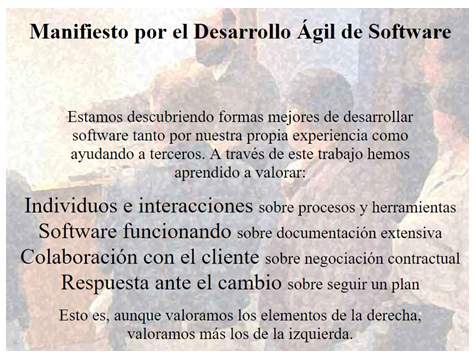
\includegraphics[width=11cm,height=8cm,]{./Images/manifiesto.png}
	\caption{Ejemplo de Clasificación de imagen de TensorFlow}
	\footnotesize Fuente: \cite{beck2001manifiesto}
	\label{manifiesto}
\end{figure}

De las metodologías ágiles conocidas, la más apropiada para el proyecto es la metodología SCRUM, debido a su seguimiento y comunicación, forzando a los miembros a un reporte diario y a un avance continuo con resultados productivos, con la posibilidad de definir metas en un tiempo específico, maximizando la efectividad de los recursos humanos.

\section{Metodología SCRUM}

La metodología SCRUM es una estrategia de gestión donde se aplica un conjunto de prácticas de manera regular para mejorar el trabajo colaborativo y obtener el mejor proyecto de Software posible\cite{scrumdiapo}.

Basado en la adaptabilidad, orientación a las personas y no los procesos y es iterativo e incremental. Requiere de la comunicación directa del cliente con el equipo desarrollador, el cual que será un miembro del equipo, al ser quien expuso, propuso y lideró el desarrollo.

La metodología SCRUM recibe los requisitos y los involucra como parte de la discusión de una reunión, para ser implementada. Se debe garantizar el desarrollo de los requisitos y permite detectar si estos producen conflictos.

\subsection{Componentes de SCRUM}

Para realizar el seguimiento de la metodología SCRUM, se requiere tomar nota de todas las decisiones realizadas, en general, la metodología fue seguida al pie de la letra, sin embargo, se destaca en Plan de Actividades, que hubo una pausa al avance del proyecto durante vasto tiempo, por tanto, se produjeron diversos cortes y extensiones de tiempo al momento de realizar las actividades, posteriormente explicado en dicho subtitulo.

\subsubsection{Roles de la Metodología SCRUM}

\begin{itemize}
	\item \textbf{Product Owner:} Es la persona que conoce el panorama completo del producto y el entorno del negocio, representa a los usuarios del producto y es responsable del seguimiento del proyecto.
	\item \textbf{SCRUM Master:} Encargado de garantizar el funcionamiento de la metodología y evaluar los procesos, es una responsabilidad del funcionamiento del modelo, es un rol flexible del que depende el éxito del proyecto.
	\item \textbf{Project Manager:} Es el encargado de dirigir el equipo a cumplir con los objetivos del equipo, se asegura de que los requerimientos se cumplan.
	\item \textbf{SCRUM Team:} Se le conoce así a los integrantes del equipo de desarrollo, que produce resultados, cuyas habilidades son aptas para el desarrollo del proyecto de Software.
\end{itemize}

Se asigno a cada uno de los integrantes del equipo un rol distintivo y aparte el rol de SCRUM Team.

\subsubsection{Sprint}

Un Sprint es también considerado una iteración y se organiza en la revisión de requisitos del usuario, el cual es la designación de los requisitos del proyecto, traduciéndose tanto en tareas de usuario como en tareas para los desarrolladores,que se distribuyen en los distintos Sprint y deben ser realizadas por el Rol de SCRUM Team. En un Sprint Backlog se realiza el seguimiento de una Sprint, es una pizarra donde se muestran las tareas a realizar en el proyecto, se detallará su funcionamiento.

\subsubsection{Requerimientos}

Los requisitos del usuario, también llamados requerimientos se los considera como un estatuto abstracto en alto nivel de un servicio. Además existen las restricciones del sistema para asegurar una funcionalidad detallada. Los requerimientos tienen las caracterizaras de ser completos, consistentes y precisos. 
La definición de requerimientos tiene que involucrar al cliente, usuario y los roles distintivos (no requiere al SCRUM Team), se debe definir e incluir en un diagrama \ref{futurediagramaderequisitos} los requerimientos para que no existan conflictos entre los interesados y los desarrolladores del proyecto.
La especificación de requerimientos se basa en la formalización y anotación escrita de los requerimientos, normalmente oficializa un contrato entre el cliente y el contratista sobre que se realizará específicamente en el proyecto para evitar demandas y huecos legales, debido a la mala interpretación o subjetividad de los requerimientos solicitados.
Finalmente se realiza la especificación del Software, que es una descripción más detallada del Software, que servirá como base para el diseño e implementación de los requerimientos, esta es manejada por el SCRUM Team.

\subsubsection{Tareas y Estimación de Poker}

Los requerimientos se transforman en tareas, básicamente es reescrito para ser entendido y manejado por el SCRUM Team que realizaran las tareas, para realizar un seguimiento del tiempo que el equipo trabaja y se toma en realizar cada tarea, se debe reunir al SCRUM Team e indagar cuanto tiempo se estimará a cada tarea, para este proyecto, se empleo el método Estimación de Poker.

Estimación de Poker es una técnica de un riesgo elevado en metodologías Ágiles, es una herramienta de asignación de tiempo requerido para realizar una tarea, que reúne a todo el SCRUM Team para realizar una estimación individual sobre la cantidad de tiempo que llevaría realizar esa actividad a través de cartas y una escala de tiempo, en este caso, de horas de 1 a 13 horas, para determinar los motivos que tiene esa persona para dar ese tiempo y llegar a un consenso sobre el tiempo requerido \cite{scrumdiapo}. Este método de estimación se empleo también para definir el tiempo de trabajo diario en que se trabajaría el proyecto.

Posteriormente, durante el proceso de elaboración de cada tarea asignada, se descubrió una realidad totalmente distinta a los números estimados, siendo indefinidamente mayores a los estimados, por tanto se tuvo que trabajar al menos 3 veces más el estimado para la mayoría de las tareas, detallado en el Product Backlog.

\subsubsection{Reuniones}

Las reuniones deben ser diarias y por Sprint, las cuales tienen el objetivo de definir cual es el trabajo que se debe realizar durante el Sprint. Para una reunión con la metodología SCRUM, deben participar todos los roles para poder generar la lista de tareas a realizar, además de determinar el objetivo de la Sprint.

Durante el transcurso del proyecto, en las reuniones diarias realizadas a horas \textbf{09:45-10:00}, se debe reportar 3 puntos del avance de los integrantes del SCRUM Team, que son el trabajo realizado, el trabajo a realizar y los problemas encontrados. Este punto de la metodología fue realizado con éxito.

\subsubsection{Sprint Backlog}

El Sprint Backlog es una pizarra donde se muestran las tareas a realizar en el proyecto, para el proyecto, se definió el uso de la herramienta \href{https://hacknplan.com/}{HacknPlan}, que es una pagina web dedicada a la administración de proyectos, brinda un servicio excepcional para la creación de un Sprint Backlog de la metodología ágil SCRUM, la cual fue recomendada por el Docente de Ingeniería de Software.
\\
La Sprint Backlog tiene 4 secciones descritas en la tabla \ref{sprintbacklog} y visualmente representadas en la figura \ref{sprintexample} que se encuentra en la sección de anexos.


\begin{table}[t]
	\begin{center}
		\begin{tabular}{| m{3cm} | m{11cm} |  }
			\hline Planificado & Las tareas traducidas para la facilidad del SCRUM Team y su resolución. \\ \hline
			En Progreso & Tareas que actualmente están siendo elaboradas por al menos un miembro del SCRUM Team. \\ \hline
			Pruebas & Tareas que han sido terminadas, pero requieren de una búsqueda de errores o aprobación del SCRUM Master. \\ \hline
			Completado & Son las tareas finalizadas, aquellas que ya no requieren cambios y han sido aprobadas por el SCRUM Master y confirmadas por el Project Manager.  \\ \hline
		\end{tabular}
		\caption{Secciones de un Sprint Backlog}
		\label{sprintbacklog}
		\footnotesize Fuente: Elaboración Propia basado en la Herramienta HacknPlan.
	\end{center}
\end{table}

Las tareas requieren de un formato para poder ser manejadas por el SCRUM Team y supervisadas por los demás roles, las secciones que componen una tarea son descritas en la tabla \ref{sprinttabla}. En la figura \ref{sprinttarea} de la sección de anexos, se puede observar un ejemplo de una tarea completada.

\begin{table}[t]
	\begin{center}
		\begin{tabular}{| m{4cm} | m{10cm} |  }
			\hline Titulo & El alias de la historia (tarea), se le asigna un nombre corto. \\ \hline
			 Importancia & Se determina su importancia en 3 niveles, bajo, normal o alta. \\ \hline
			 Estimación Inicial & Se determina el tiempo que toma la actividad, previamente definido con Planning Poker \\ \hline
			 Descripción & Lo que se busca realmente, el requerimiento funcional que se necesita para la elaboración de la tarea, se detalla lo que se requiere, esta sección es empleada solo para las tareas de programación. \\ \hline
			 Comentarios & Se describen los avances, problemas encontrados y varios a medida que se desarrolla o termina la tarea. \\ \hline
			Registro de trabajo  & Acompañado de un comentario donde se registra que se hizo, se anota cuanto tiempo estuvieron que miembros del SCRUM Team en la tarea. \\ \hline
		\end{tabular}
		\caption{Secciones de una tarea dentro del Sprint Backlog}
		\label{sprinttabla}
		\footnotesize Fuente: Elaboración Propia basado en la Herramienta HacknPlan.
	\end{center}
\end{table}

\subsubsection{Product Backlog}

El Product Backlog es una lista de requisitos o tareas que representa la visión y expectativa del cliente respecto a objetivos y entregas del proyecto. Se debe mencionar el valor y el costo de su finalización. Se puede observar el Product Backlog en la tabla \ref{productbacklog}.

En la tabla, se observan los campos:
\begin{itemize}
	\item ID como identificador de la tarea, debe ser único.
	\item Tarea, que indica el título dado en Sprint Backlog para facilitar su comprensión.
	\item Estado(Sprint), si ha de estar Planificada, En Proceso o Hecho (Sprint en que se realizo) o si fue Descartado.
	\item Valor, el valor designado a cada actividad realizada, en total se asignan 1000 puntos a su finalización
	\item Estimado Inicial, la valoración de las tareas que se mide en horas requeridas.
	\item Factor Ajuste, determina el fallo que se debe aumentar al tiempo original, se le suma al Valor Estimado en función $Valor Estimado = Valor Estimado + Valor Estimado * Factor de Ajuste$
	\item Ajustado, es la valoración de las tareas posteriormente al ser más realistas sobre el tiempo requerido para resolverlo.
	\item Sprint, que señala el número de Sprint en que fue realizada
	\item  Prioridad, al ser una metodología ágil, se reconoce que las tareas pueden ser más relevantes unas que otras, en este caso, Baja, Normal y Alta.

\end{itemize}
La Tarea es el nombre dado a las tareas distribuidas al SCRUM Team, formuladas a partir de los requerimientos del cliente.
El valor de las tareas se distribuirá de un valor total de 1000 puntos, se determinara una cuarta parte a la redacción del informe, una cuarta parte a la investigación dedicada requerido para poder hacer posible el proyecto y el resto lo determinará el rol de Product Owner.
El Estimado Inicial es definido con la Estimación de Poker previamente mencionada.
Redactar en la tabla \ref{productbacklog} engloba la redacción del informe y el tiempo estimado de cada tarea de redacción, el Redactar hace referencia a los títulos de cada parte del informe.
En Redactar Parte 1, están los títulos de Objetivos, Estudio de Diagnóstico, Marco Teórico, Estudio de Alternativas, Plan de Actividades
En Redactar Parte 2, están los títulos de Metodología, Diseño, Conclusiones, Recomendaciones, dentro de la metodología se lleva a cabo la tarea de Seguimiento de Product Owner.
En Redactar Parte 3, están los títulos de Introducción, Anexos, Glosario, Revisión de ortografía y Resumen.
\restoregeometry
\newgeometry{left=0.5cm,bottom=.25cm}
\begin{landscape}
\begin{table}[t]
	\begin{center}
		\begin{tabular}{| c | c | c | c | c | c | c | c | c |}
			\hline
			\multicolumn{9}{ |c| }{Product Backlog} \\ \hline
			ID & Tarea & Estado(Sprint) & Valor & Estimado Inicial (h)& Factor Ajuste & Ajustado(h) & Sprint & Prioridad \\ \hline
			T-0 & Redactar Parte 1 & Hecho(1) & 50 & 18 & 1.5 & 40 & 1 & Normal \\ \hline
			T-1 & Redactar Parte 2 & (2) & 100 & 20 &  &  & 2 & Normal \\ \hline
			T-1 & Redactar Parte 3 & (3) & 100 & 9 &  &  & 3 & Normal \\ \hline
			T-2 & Investigación de Herramientas & Hecho(1) & 250 & 24 & 3.0 & 96 &  1 & Normal \\ \hline
			T-3 & Manipulación de Herramientas & Hecho(1) &  & 12 & 1.0 & 24 & 1 & Normal \\ \hline
			T-4 & Modificación de GUI & Hecho(1) &  &  & &  & 1 & Baja \\ \hline
			T-5 & Mostrar Video a Copiar en la Pantalla & Hecho(1) &  &  & &  & 1 & Alta \\ \hline
			T-6 & Lectura de Movimientos del Usuario & Hecho(1) &  &  & &  & 1 & Alta \\ \hline
			T-7 & Redimension de Imagen para Comparar & Hecho(1) &  &  & &  & 1 & Alta \\ \hline
			T-8 & Menú y Boton Play de Redireccionamiento & Hecho() &  &  & &  &  & Normal \\ \hline
			T-9 & Calificación de Movimientos & Hecho(2) &  & 10 &  &  & 2 & Alta \\ \hline
			T-10 & Mostrar acciones a copiar & Hecho() &  & 3 & &  &  & Alta \\ \hline
			T-15 &  & Hecho() &  &  & &  &  & Normal \\ \hline
			 & Entrega final & & 1000 &  &  & 900 &  &  \\ \hline
		\end{tabular}
		\caption{Product Backlog}
		\label{productbacklog}
		\footnotesize Fuente: Elaboración propia
	\end{center}
\end{table}
\end{landscape}
\restoregeometry

\subsubsection{Gráfica Burn-Up}

Es una herramienta de seguimiento que se usa en la metodología ágil SCRUM, sirve para determinar el tiempo estimado del proyecto en general, para tener una referencia visual de cuanto progreso se realizo realmente, se establecieron los siguientes puntos:

\begin{itemize}
	\item Versión 0.1: Tiempo en que se estima tendrá una demo para presentar.
	\item Horas Estimadas de Trabajo: Cantidad de horas totales estimadas para la realización del proyecto.
	\item Horas Acumuladas: Cantidad de horas registradas durante los Sprint para cada tarea que tiene progreso, no necesariamente terminadas para sumarlas a la gráfica. 
	\item Trayectoria Estimada: La estimación optimista de la distribución de horas, determina la trayectoria de las horas acumuladas deseada.
\end{itemize}

Para estimar la cantidad de horas de trabajo se empleará un calculo simple.
 Primero se estiman 3 horas en promedio en un rango de 2 a 5 horas de trabajo diario mientras la Sprint este activa, se toma en cuenta que se trabajaran todos los. La estimación de tiempo toma en cuenta que la fecha de inicio del proyecto es el 17 de Septiembre y la fecha de entrega estimada es el 14 a 17 de Diciembre, determinando un total de 88 días mínimo, se las multiplica y redondea al dígito más grande como se ve en la ecuación \ref{eqn:horasestimadas}.
 
\begin{equation} 
\label{eqn:horasestimadas} 
	792 \text{ Horas Estimadas de Trabajo} = 3 \text{ Horas Diarias} * 3 \text{ Personas} * 88 \text{ Días disponibles}	
\end{equation}

La cantidad de horas estimadas se redondea a 800 horas, este es un calculo pesimista, tomando en cuenta que el desconocimiento inicial de las herramientas con las que se trabajan y el tiempo que tome resolver problemas sea muy elevado, que durante el desarrollo se demuestra que es necesario.

\subsubsection{Gráfica Burn-Down}

Es una herramienta de seguimiento que se usa en la metodología ágil SCRUM, sirve para determinar el tiempo estimado que se tiene en total para cada tarea y todas las tareas, para tener una referencia visual de cuanto progreso se ha completado en comparación al ideal, se establecieron los siguientes puntos:

\begin{itemize}
	\item Remanente Ideal: En una trayectoria descendiente deseada para estimar resultados, se observa la cantidad de horas que faltan para  llegar a la meta.
	\item Esfuerzo Remanente: Es la cantidad de horas que todavía faltan por registrar por parte del SCRUM Team.
	\item Tareas Remanentes: Cantidad de tareas totales de las Sprint que faltan por completar.
	\item Tareas Completadas: Tareas realizadas durante ese espacio de tiempo especifico. 
\end{itemize}
				





Se refiere a usar Metodologia Scrum o redactar de como organizamos la metodologia, preguntar
\chapter{Análisis y Desarrollo del Diseño del Sistema Interactivo}

El diseño propuesto es elaborado a partir de los requerimientos recopilados por parte de un cliente inicial externo a la universidad y se busca satisfacer las necesidades del usuario que lo emplee. La propuesta será diseñada a partir de las bases de la ingeniería de Requerimientos aplicada en la metodología ágil SCRUM.

La ingeniería de requerimientos del proyecto implica establecer lo que el cliente y usuario requiere del sistema interactivo \cite{scrumdiapo}, además de la funcionalidad esperada del proyecto, se debe definir, especificar y validar los requerimientos para poder aprobar su elaboración.

De la siguiente manera la solicitud del cliente inicia con un pedido ambiguo y coloquial por parte del instructor de artes marciales de uno de los integrantes del grupo al compartir su idea con el, juntos anotaron sus pensamientos con las siguientes palabras: ``Me gustaría un juego con el cual pueda entrenar las poses y técnicas básicas de Karate siguiendo lo que hace en la pantalla y que me diga si lo hago bien o mal, pero no tengo un Kinect o una consola para jugar, solo mi laptop", a lo cual el estudiante añadió ``Pero también sería genial que puedas bailar e imitar lo que hace la gente, si va por esa línea, podrías generalizarlo para atraer más público". Es de conocimiento general que las ideas suelen venir de lugares inesperados, en este caso, fue una conversación coloquial entre dos conocidos lo que inspiro el proyecto, a partir de esas palabras, se determina la base del proyecto, por tanto, se debe recabar entre las frases, se las dividirá e interpretará dividiéndolo en 4 secciones como se ven en la tabla \ref{requerimientos}. Si bien, el instructor perdió el interés en el proyecto con el pasar del tiempo, el estudiante tomará el rol de cliente para el desarrollo del sistema interactivo.


\begin{table}[t]
	\begin{center}
		\begin{tabular}{|m{7cm}|m{8cm}|}
			\hline Solicitud en lenguaje coloquial & Interpretación inicial como requerimiento \\ \hline
			\multirow{3}{7cm}{Me gustaría un juego con el cual pueda entrenar las poses y técnicas básicas de Karate siguiendo lo que hace en la pantalla.}
			& Desarrollar un sistema interactivo.\\ 
			& Existe un vídeo o instrucción en una pantalla para poder entrenar artes marciales.\\ & El usuario debe moverse acorde lo visto en la pantalla. \\ \hline
			Que me diga si lo hago bien o mal. & Se requiere de un sistema de calificaciones para los movimientos hechos por el usuario. \\ \hline
			No tengo un Kinect o una consola para jugar, solo mi laptop. & Tiene que funcionar en una laptop. \\ \hline
			Sería genial que puedas bailar e imitar lo que hace la gente. & No debe limitarse a artes marciales. \\ \hline
		\end{tabular}
		\caption{Interpretación de la solicitud inicial del cliente}
		\label{requerimientos}
		\footnotesize Fuente: Elaboración Propia.
	\end{center}
\end{table}

Posteriormente, se vio conveniente ser capaz de usar vídeos proporcionados por el usuario para poder crear niveles propios, ya que si inicialmente el instructor lo deseaba para entrenar poses y técnicas de Karate, él habría provisto de los vídeos, sin embargo, se emplearan recursos de terceros para realizar las pruebas del prototipo que se desarrolle.

\section{Análisis de Requerimientos}

En un principio, se debe definir como se llamará a los distintos vídeos que se desean imitar, formalmente se lo conocerá en el contexto como: \textbf{Mapa, mapa es un conjunto de poses que el usuario debe imitar en tiempo cronometrado de un determinado vídeo}. 

Se desarrolla un sistema interactivo que permite al usuario poder jugar distintos mapas y además crear mapas propios, para ello se requieren dos funciones fundamentales.

\begin{itemize}
	\item Play: Refiere al acto de entrar a una lista de mapas de usuario, donde se seleccionará un mapa y se realizará el seguimiento de las acciones provistas por el sistema interactivo a imitar.	
	\item Crear un nuevo mapa: Término dado a la elaboración de mapas, donde el usuario provee un vídeo que quiera convertir en un mapa del sistema interactivo.
\end{itemize}

Se debe dar a conocer la forma en que los usuarios interactúan con el sistema interactivo, definir ciertas limitación, realizar consideraciones respecto a la interfaz gráfica y a las modificaciones externas del producto.

\subsubsection{Características de Usuario}

El sistema interactivo contará con una categoría Apto para todo público según el sistema PEGI y Early Childhood en el sistema ESRB, por tanto los usuarios puede ser cualquier persona mayor a los 3 años que pueda emplear el sistema interactivo. Sin embargo, debido a que está diseñado para realizar actividad física, se recomienda un control de salud previo uso para no resultar herido o lastimado en caso de ser mayor de edad o tener problemas que limiten las actividades físicas.
La creación de los mapas requiere de la lectura de un ligero manual de usuario y perseverancia para la actividad tediosa, por tanto, si bien puede hacerlo cualquiera, es recomendado que lo hagan mayores de 12 años.


\subsection{Requerimientos Funcionales}

Los requerimientos funcionales hacen referencia a todas las funcionas que tiene disponible el usuario para realizar dentro del sistema interactivo, según los módulos y componentes externos que lo integran. Se mencionaron dos requerimientos funcionales, los cuales, se descomponen en:

\subsubsection{Play}

\begin{enumerate}
	\item Jugar: La opción de afirmar que se jugara, debe dirigirte a seleccionar el mapa deseado.
	\item Opciones: El usuario es capaz de interactuar con las opciones descritas en 3 y 4.
	\item Subir/Bajar el volumen: Una de las opciones es poder subir y bajar el volumen del audio del vídeo en una escala de 0 a 1.
	\item Cambiar la resolución: Una opción más, esta permitirá el cambio del tamaño de la ventana del sistema interactivo, debe tener múltiples resoluciones disponibles.
	\item Seleccionar el nivel deseado: Una vez se elije jugar, el usuario puede seleccionar el mapa con el que interactuar.
	\item Salir: La opción de dejar de ejecutar el sistema interactivo.
	\item Mostrar calificación al terminar el mapa: Un usuario debe ser capaz de visualizar la calificación que va acumulando a medida que realiza el nivel.
	\item Salir del mapa: La capacidad del usuario para interrumpir el seguimiento del mapa.
	\item Pausar juego: El usuario debe ser capaz de detener el mapa en proceso cuando este haya sido selecto para ejecutar.
\end{enumerate}

\subsubsection{Crear un nuevo mapa}

Para la creación de un mapa, se tiene que seguir una serie de 5 pasos que involucran al usuario:

\begin{enumerate}
	\item Ejecutar Script de conversión de vídeo a JSON e imágenes en formato JPG: El usuario selecciona un vídeo, usará un Script para el primer paso de conversión a un mapa.
	\item Ejecutar Script de JSON a .txt: Posteriormente, se vuelve a usar otro Script para una segunda conversión a un formato intuitivo de entender para el usuario
	\item Selección manual de poses: Para crear un mapa, solo se requieren poses específicas para cada movimiento, se borran las que se consideren redundantes de entre los txt.
	\item Guardar el resultado en una carpeta designada para los mapas del usuario: Se guarda en una carpeta el nuevo mapa, en preparación al siguiente paso.
	\item Añadir un margen de tiempo para realizar las poses: Todas las poses de cada nivel tienen que tener una variable que determine el tiempo límite que se tiene para realizar esa acción. 
\end{enumerate}

\subsection{Requerimientos No Funcionales}

Los requerimientos no funcionales indican los limites del sistema o el proceso de desarrollo, entre ellos se emplearan:

\begin{enumerate}
	\item Interfaz Gráfica de Usuario: Desarrollar una interfaz de usuario, para poder emplear fácilmente los requerimientos funcionales, el sistema interactivo de una manera más efectiva.
	\item Funcionalidad: Que la capacidad del sistema interactivo sea capaz de funcionar acorde lo mencionado en los requerimientos funcionales.
	\item Confiabilidad: Inicialmente, el plug-in de Unity tiene una tendencia a cerrarse repentinamente y al abrirlo por primera vez viene con archivo corruptos que se tienen que arreglar, se espera solucionar o al menos reparar esta debilidad de ser posible.
	\item Intuitividad: Se espera que el cliente sea capaz de entender que actividad hacer con solo ver las funciones disponibles en la interfaz gráfica.
\end{enumerate}
\newpage
\subsection{Funcionalidad Esperada del Sistema Interactivo}

Se prepara un resumen visual de los requerimientos solicitados por el cliente, donde se separan los dos tipos de usuario que emplearán el producto final

\begin{figure}[h]
	\centering
	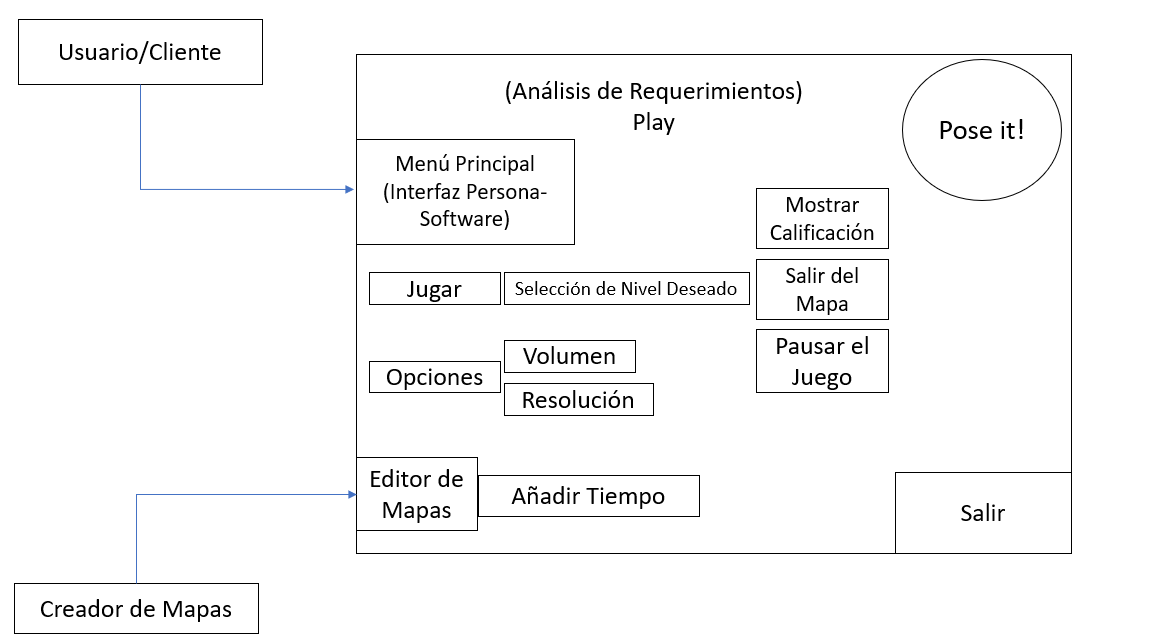
\includegraphics[width=16cm,height=10cm,]{./Images/requerimientosgraficaposeit.png}
	\caption{Ilustración de Requerimientos en la GUI}
	\footnotesize Fuente: Elaboración Propia
	\label{requerimientosgrafico}
\end{figure}

\clearpage
\subsection{Diagrama de Flujo de Datos}

Un diagrama de flujo de datos provee una función gráfica de los datos que se tienen dentro de un sistema de información, esencialmente se puede disponer de una vista a las variables y métodos esenciales, en este caso se aprecia el diagrama presentado por OpenPose que será modificado en una fase posterior del proyecto.

\begin{figure}[h]
\centering
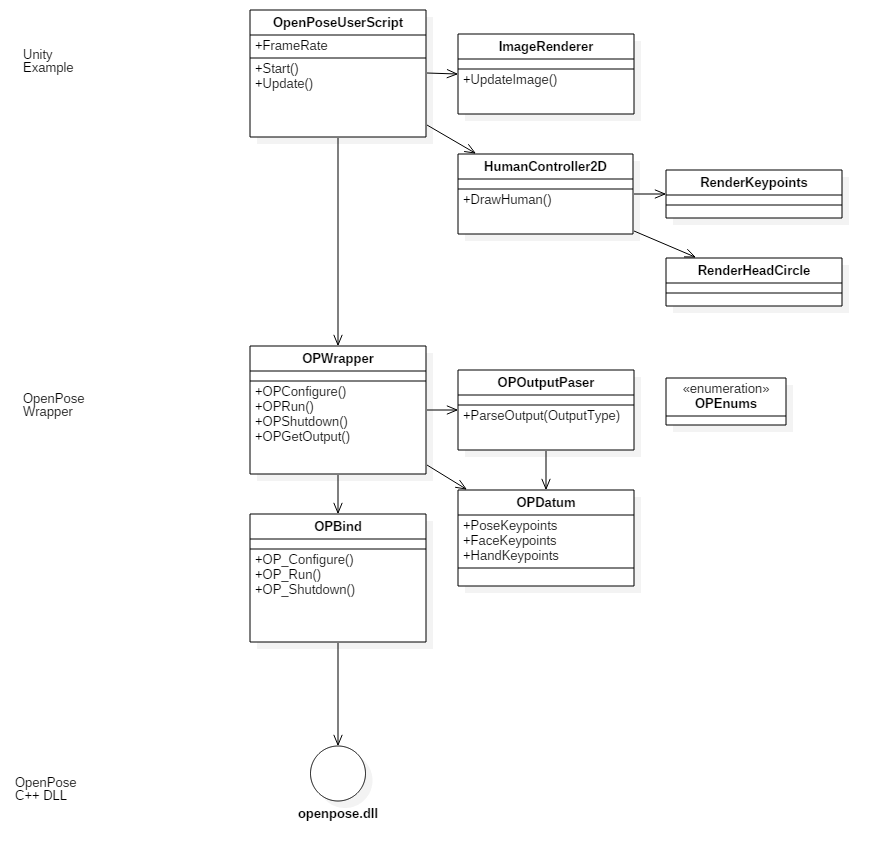
\includegraphics[width=14cm,height=14cm,]{./Images/futurediagramaderequisitos.png}
\caption{Diagrama de Datos de Flujo}
\footnotesize Fuente: Versión original del Diagrama de Flujo de Datos OpenPose \cite{8765346}
\label{dfd}
\end{figure}



\chapter{Plan de Actividades}

El desarrollo del proyecto inicia oficialmente el día 17 de Septiembre, con la definición del perfil del proyecto por parte del grupo de estudiantes.

El desarrollo fue interrumpido debido a la concentración del equipo en otras actividades, que exigió el 100\% del tiempo libre y de estudio y progreso en el proyecto, siendo más específicos la materia de Aplicación con Redes, estimando entre 4 a 8 horas diarias (incluyendo fines de semana) de exigencia entre estudio y practicas para mantener el ritmo solo a esa materia. Debido a ello, desde la fecha 18 de septiembre del 2020, a la fecha 4 de noviembre del 2020, el progreso fue mínimo, reduciéndose a la búsqueda de API's y herramientas, así como la redacción base del proyecto y la oficialización interna del producto deseado.

La metodología SCRUM fue inicializada oficialmente y de manera constante el día 10 de Noviembre del 2020, planteando un rango de horas de trabajo de 2 a 5 horas diarias (incluyendo fines de semana), con la finalización del Sprint los sábados por la mañana, a menos que sea una entrega de avance, la cual requerirá de una finalización del Sprint hasta donde se encuentra el proyecto en ese momento.


\restoregeometry
\newgeometry{left=1.3cm,bottom=1.3cm}
\begin{landscape}
	\subsection{Cronograma}
	\begin{ganttchart}[
		hgrid=true,
		vgrid={*1{red, dashed}, *1{green, dashed}, *1{blue, dashed}},
		bar/.append style={fill=red!50},
		x unit=2.5mm,
		time slot format=isodate
		]{2020-09-17}{2020-12-19}
		\gantttitlecalendar{month=name, , week=1, weekday} \\
		\ganttbar{T1}{2020-09-17}{2020-09-26} \\
		\ganttbar{T2}{2020-09-17}{2020-11-05} \\
		\ganttbar{T3}{2020-10-01}{2020-12-03} \\
		\ganttbar{T4}{2020-11-06}{2020-12-03} \\
		\ganttbar{T5}{2020-12-04}{2020-12-11} \\
		\ganttbar{T6}{2020-12-04}{2020-12-11} \\
		\ganttbar{T7}{2020-12-12}{2020-12-19} 		
	\end{ganttchart}


Cada TX representa un título
\begin{itemize}
	\item T1 \emph{Redacción del Perfil}.
	\item T2 \emph{Investigación}.
	\item T3 \emph{Redacción del documento}.
	\item T4 \emph{Implementación de la aplicación}.
	\item T5 \emph{Revisión final del documento}.
	\item T6 \emph{Revisión final de la aplicación}.
	\item T7 \emph{Redacción de la presentación}.
\end{itemize}
\end{landscape}


\restoregeometry

\chapter{Evaluación Financiera Comparada}



\chapter{Conclusiones}


Durante el trayecto del proyecto se realizaron diferentes actividades y seguimientos de las mismas, además de la aplicación de herramientas externas apropiadamente empleadas y una metodología ágil en su mayoría, si bien se tuvo dificultades de gran proporción con la estimación de tiempo, a fin de cuentas, no fue un factor que determine el fracaso del proyecto, es más, se afirma que los objetivos fueron cumplidos de acuerdo al producto mínimo viable establecido en delimitación.

En función a los objetivos específicos, a lo largo del desarrollo e implementación del prototipo diseñado, se llega a la conclusión siguiente.

Respecto al primer objetivo específico, utilizar Software existente para el seguimiento corporal utilizando una cámara, en el estudio de alternativas se observan varias herramientas de Software que posibilitaban el desarrollo del proyecto, al emplear OpenPose, la mejor alternativa, que sirve para el seguimiento corporal y se la empleo utilizando cámaras web, siendo las pruebas con el prototipo realizadas empleando diferentes modelos de cámara Web, se determina que el objetivo específico es cumplido satisfactoriamente.
\\

Respecto al segundo objetivo específico, implementar una función para registrar mapas de movimiento propios del usuario,


Respecto al tercer objetivo específico,proveer una alternativa factible al mercado de sistemas interactivos con Body Tracking tales como Just Dance.


Respecto al objetivo general.


Desarrollo de un sistema interactivo con Body Tracking, empleando una cámara común para entrenamiento, seguimiento de posiciones, técnicas de arte marcial y baile.

Presentación de las principales conclusiones
Relación de los objetivos propuestos y los objetivos
alcanzados
\bibliographystyle{plain}
\bibliography{bibliografia}
\chapter{Recomendaciones}
Indicación de recomendaciones con relación a la
implementación futura de la solución propuesta o
de mejoras posibles relacionadas a la
implementación (si es que ésta se llevó a cabo)
\chapter{Anexos}


para la bibliografia

Relación numerada o alfabética (Nombre, Año) de
las referencias bibliográficas de todos los aportes
tomados de terceros y citados en el texto del
proyecto 
2 o mas paginas



Presentación estructurada de la información
imprescindible de respaldo, que se retira del texto
principal sólo para facilitar la lectura ágil del
documento. 

variable




\end{document}

